% =========================================================================
% Calango User Guide
% Build:  pdflatex calango_user_guide.tex   (run twice for the ToC)
% Style follows docs/packaging.tex, extended with callouts and diagrams.
% =========================================================================
\documentclass[11pt,a4paper]{report}

\usepackage[margin=2.5cm,headheight=26pt,headsep=16pt]{geometry}
\usepackage{lmodern}
\usepackage[T1]{fontenc}
\usepackage[utf8]{inputenc}
\usepackage{microtype}
\usepackage{amsmath}
\usepackage{graphicx}
\usepackage{xcolor}
\usepackage{booktabs}
\usepackage{longtable}
\usepackage{array}
\usepackage{listings}
\usepackage{enumitem}
\usepackage{titlesec}
\usepackage{fancyhdr}
\usepackage{tcolorbox}
\usepackage{tikz}
\usepackage{needspace}
\usepackage{parskip}
\usepackage[colorlinks=true,linkcolor=calangoteal,urlcolor=calangoteal,
            citecolor=calangoteal]{hyperref}

\tcbuselibrary{skins,breakable}
\usetikzlibrary{positioning,fit,backgrounds}

% --- Brand palette (shared with docs/packaging.tex) ------------------------
\definecolor{calangoteal}{RGB}{0,110,110}
\definecolor{calangodark}{RGB}{30,34,40}
\definecolor{codebg}{RGB}{245,246,248}
\definecolor{shadegray}{RGB}{90,96,104}
\definecolor{tipgreen}{RGB}{22,120,80}
\definecolor{warnamber}{RGB}{176,125,42}
\definecolor{panelgray}{RGB}{232,235,239}

% --- Chapter / section typography -----------------------------------------
\titleformat{\chapter}[display]
  {\bfseries\color{calangodark}}
  {\raggedright\large\color{shadegray}\MakeUppercase{\chaptertitlename}\ \Huge\color{calangoteal}\thechapter}
  {6pt}
  {\Huge\raggedright}
  [\vspace{4pt}{\color{calangoteal}\rule{\textwidth}{1.6pt}}]
\titlespacing*{\chapter}{0pt}{-18pt}{22pt}

\titleformat{\section}
  {\Large\bfseries\color{calangodark}}
  {\textcolor{calangoteal}{\thesection}}{0.8em}{}
  [\vspace{-6pt}{\color{calangoteal!35}\rule{\textwidth}{0.8pt}}]
\titleformat{\subsection}
  {\large\bfseries\color{calangodark}}
  {\textcolor{calangoteal}{\thesubsection}}{0.8em}{}
\titleformat{\subsubsection}
  {\normalsize\bfseries\color{calangodark}}
  {\textcolor{calangoteal}{\thesubsubsection}}{0.7em}{}
\titlespacing*{\section}{0pt}{18pt}{10pt}
\titlespacing*{\subsection}{0pt}{12pt}{6pt}

\setcounter{tocdepth}{1}
\setcounter{secnumdepth}{3}

% --- Running header / footer ----------------------------------------------
\pagestyle{fancy}
\fancyhf{}
\fancyhead[L]{\raisebox{-4pt}{%
  
\includegraphics[height=18pt]{../../assets/.internal/logo_light.png}}}
\fancyhead[R]{\small\color{shadegray}\nouppercase{\leftmark}}
\fancyfoot[L]{\small\color{shadegray}Calango User Guide}
\fancyfoot[R]{\small\color{shadegray}\thepage}
\renewcommand{\headrulewidth}{0.8pt}
\renewcommand{\headrule}{{\color{calangoteal}%
  \hrule width\headwidth height\headrulewidth}}
\renewcommand{\footrulewidth}{0pt}
\renewcommand{\chaptermark}[1]{\markboth{\thechapter.\ #1}{}}
\fancypagestyle{plain}{\fancyhf{}%
  \fancyfoot[R]{\small\color{shadegray}\thepage}%
  \renewcommand{\headrulewidth}{0pt}}

% --- Code listings: teal accent bar ---------------------------------------
\lstdefinestyle{shell}{
  basicstyle=\ttfamily\small,
  backgroundcolor=\color{codebg},
  frame=leftline,
  framerule=2.4pt,
  rulecolor=\color{calangoteal},
  framesep=8pt,
  xleftmargin=12pt,
  xrightmargin=6pt,
  aboveskip=10pt,
  belowskip=10pt,
  breaklines=true,
  breakatwhitespace=true,
  postbreak=\mbox{\textcolor{shadegray}{$\hookrightarrow$}\space},
  columns=fullflexible,
  keepspaces=true,
  showstringspaces=false,
  upquote=true,
}
\lstset{style=shell}

% --- Semantic inline markup ------------------------------------------------
\newcommand{\file}[1]{\texttt{#1}}
\newcommand{\opt}[1]{\texttt{#1}}
% A UI control (button, field, checkbox label).
\newcommand{\ui}[1]{\textcolor{calangodark}{\textsf{\textbf{#1}}}}
% A menu path: \menu{Analysis}{Raman Modes}
\newcommand{\menusep}{\,\textcolor{calangoteal}{$\rangle$}\,}
\newcommand{\menu}[1]{\textsf{\textbf{\textcolor{calangodark}{#1}}}}
% A keyboard key.
\newcommand{\kbd}[1]{%
  \tikz[baseline=(k.base)]{\node[draw=shadegray,fill=panelgray,rounded corners=2pt,
    inner xsep=4pt,inner ysep=1.5pt,line width=0.4pt](k){\small\textsf{#1}};}}

% --- Callout boxes ---------------------------------------------------------
\newtcolorbox{calnote}[1][]{%
  breakable, enhanced, colback=calangoteal!5, colframe=calangoteal,
  boxrule=0pt, leftrule=3pt, arc=1pt, left=8pt, right=8pt, top=6pt, bottom=6pt,
  fonttitle=\bfseries\small, title={Note}, coltitle=calangoteal,
  attach title to upper=\par\vspace{2pt}, #1}
\newtcolorbox{caltip}[1][]{%
  breakable, enhanced, colback=tipgreen!5, colframe=tipgreen,
  boxrule=0pt, leftrule=3pt, arc=1pt, left=8pt, right=8pt, top=6pt, bottom=6pt,
  fonttitle=\bfseries\small, title={Tip}, coltitle=tipgreen,
  attach title to upper=\par\vspace{2pt}, #1}
\newtcolorbox{calwarn}[1][]{%
  breakable, enhanced, colback=warnamber!7, colframe=warnamber,
  boxrule=0pt, leftrule=3pt, arc=1pt, left=8pt, right=8pt, top=6pt, bottom=6pt,
  fonttitle=\bfseries\small, title={Requires}, coltitle=warnamber,
  attach title to upper=\par\vspace{2pt}, #1}

% Compact description lists used throughout the reference sections.
\setlist[description]{style=unboxed,leftmargin=1.2em,itemsep=3pt,topsep=4pt}
\setlist[itemize]{itemsep=2pt,topsep=4pt}
\setlist[enumerate]{itemsep=3pt,topsep=4pt}

\begin{document}

% =========================== TITLE PAGE ===================================
\begin{titlepage}
\centering
\vspace*{2.0cm}

\includegraphics[width=0.55\textwidth]{../../assets/.internal/logo_light.png}\par
\vspace{1.3cm}
{\color{calangoteal}\rule{0.74\textwidth}{1.6pt}}\par
\vspace{0.9cm}
{\Huge\bfseries User Guide\par}
\vspace{0.5cm}
{\Large Visual atomistic modeling, simulation and analysis\par}
\vspace{0.9cm}
{\color{calangoteal}\rule{0.74\textwidth}{1.6pt}}\par
\vspace{1.5cm}
{\large\bfseries Leandro Seixas\par}
\vspace{0.3cm}
{\large\color{shadegray}Seixas Research\par}
\vfill
{\large July 2026 --- Calango 26.7.26\par}
\vspace*{1.2cm}
\end{titlepage}

\chapter*{About this guide}
\addcontentsline{toc}{chapter}{About this guide}
\markboth{About this guide}{}

Calango is a desktop application for building, visualizing, simulating and
analysing atomic structures. It pairs a C++20 / OpenGL core --- fast enough
to orbit tens of thousands of atoms in real time --- with an embedded
CPython interpreter running the Atomic Simulation Environment (ASE), so
every structure you see on screen can be handed to a real calculator
without leaving the program.

This guide is written for the person using Calango, not the person
building it. It walks through the workspace, then covers each menu in the
order you are likely to need it: getting data in, building and editing
structures, making them look right, running simulations locally or on a
cluster, and analysing the results. Chapter~\ref{ch:reference} is a
reference you can jump straight to --- keyboard shortcuts, the complete
menu map, file formats and troubleshooting.

\section*{Conventions}

\begin{description}
  \item[\menu{Analysis}\menusep\menu{Raman Modes}] A menu path. Each
    \menusep{} step is one level deeper.
  \item[\ui{Compute}] A button, field, checkbox or tab label exactly as it
    appears in the interface.
  \item[\kbd{Ctrl}+\kbd{R}] A keyboard shortcut. On macOS, \kbd{Ctrl}
    means \kbd{Cmd} wherever the shortcut is a standard editing action
    (open, save, quit, undo); single-letter viewport shortcuts have no
    modifier on any platform.
  \item[\file{run.py}] A file, directory or path.
\end{description}

Three kinds of callout appear throughout:

\begin{calnote}
Background you do not strictly need, but that explains why something
behaves the way it does.
\end{calnote}

\begin{caltip}
A shortcut or working habit that saves time.
\end{caltip}

\begin{calwarn}
An external dependency --- a Python package, a solver binary, a network
connection --- that the feature cannot work without.
\end{calwarn}

\Needspace{6\baselineskip}
\section*{Version}

This guide documents Calango \textbf{26.7.83}. The version you are running
is shown in \menu{Help}\menusep\menu{About Calango}, together with the
Python and ASE versions actually in use --- worth checking first whenever
something behaves unexpectedly.


\tableofcontents

\chapter{Getting Started}
\label{ch:getting-started}

\section{Installing Calango}

Calango ships as a native installer for each desktop platform:

\begin{description}
  \item[macOS] A drag-and-drop \file{.dmg}. Mount it and drag
    \file{calango.app} onto the \file{Applications} shortcut.
  \item[Linux] A Debian package. Install it with \opt{apt} so dependencies
    resolve automatically:
    \begin{lstlisting}
sudo apt install ./calango_26.7.26_amd64.deb
    \end{lstlisting}
    The package registers a desktop launcher, an application icon, and a
    MIME type for \file{.calproj} files, so double-clicking a project in
    your file manager opens the workspace.
\end{description}

Building from source is covered in the companion \emph{Calango Packaging
Guide} (\file{docs/packaging.pdf}), which also documents how the installers
are produced.

\section{The Python environment}
\label{sec:python-env}

Calango embeds a CPython interpreter and drives ASE through it. Almost
everything that touches chemistry --- reading a CIF, building a slab,
running a calculation --- goes through that interpreter, so pointing
Calango at a Python that has ASE installed is the single most important
piece of setup.

\subsection{How the interpreter is chosen}

An embedded interpreter does not inherit an activated virtual environment
the way a shell does, so Calango resolves one explicitly, in this order:

\begin{enumerate}
  \item \opt{\$CALANGO\_PYTHON} --- an explicit path to a Python
    executable. Highest priority; use this to override everything else.
  \item \opt{\$VIRTUAL\_ENV} --- an activated virtual environment, if
    Calango was launched from that shell.
  \item A Python bundled inside the installed application
    (\file{Contents/Resources/python} on macOS,
    \file{\textless prefix\textgreater/lib/calango/python} on Linux), when the installer
    was built with one.
  \item The interpreter the build was configured against.
\end{enumerate}

\begin{calwarn}
Calango needs \texttt{ase} and \texttt{numpy} at minimum. Individual
features add their own requirements: \texttt{spglib} (symmetry, Raman
modes), \texttt{paramiko} (remote access), \texttt{pillow} /
\texttt{imageio} / \texttt{imageio-ffmpeg} (animation export),
\texttt{mace-torch} (ML potentials), \texttt{gpaw} (DFT bands and PDOS). A complete environment:
\begin{lstlisting}
python3 -m venv .venv
.venv/bin/pip install ase numpy spglib paramiko pillow imageio \
                      imageio-ffmpeg
\end{lstlisting}
\end{calwarn}

\subsection{Checking the environment}

Before opening any structure, confirm the interpreter is the one you
expect:

\begin{lstlisting}
calango --probe-python
\end{lstlisting}

This runs headlessly and prints the resolved interpreter, the Python
version and the ASE version, exiting with status 0 only when ASE imports
successfully. It is the first thing to run when structure loading fails.

If ASE cannot be imported at launch, Calango still starts --- so you can
adjust settings --- but structure I/O and job features are disabled, and a
warning explains how to point at a working interpreter.

\begin{caltip}
Simulation jobs do not have to use the embedded interpreter. The
calculator, phonon and band-structure dialogs each carry an
\ui{Execution Environment} selector that routes the job to any Conda
environment or interpreter path (Section~\ref{sec:exec-env}). This is how
you keep, say, a GPAW environment separate from the one Calango itself
uses.
\end{caltip}

\subsection{The environment file}
\label{sec:envfile}

At launch Calango reads an environment file --- \file{\textasciitilde/.env}
by default --- and exports \opt{MP\_API\_KEY}, the Materials Project API
key, into the process environment. A key already present in your shell
takes precedence at startup.

Point Calango at a different file, or re-read it on demand, in
\menu{Edit}\menusep\menu{Preferences}. The dialog reports whether the file
exists and whether it actually defines a key. The same controls are
mirrored in the \ui{Materials Project} tab of the database browser.

\section{First launch}

Calango opens with an empty workspace. Three quick ways to get something
on screen:

\begin{enumerate}
  \item \menu{File}\menusep\menu{Open}\menusep\menu{Structure} and pick any
    structure file (Section~\ref{sec:formats} lists the formats).
  \item \menu{Build}\menusep\menu{From Database} and load one of the
    bundled presets --- diamond, bulk and monolayer MoS$_2$, graphene,
    benzene, naphthalene, coronene.
  \item Pass a file on the command line: \lstinline|calango structure.cif|.
    Each file argument opens in its own tab; a \file{.calproj} argument
    restores a whole saved session.
\end{enumerate}

\chapter{The Workspace}
\label{ch:workspace}

\section{The 12-zone grid}

Calango opens into a fixed default arrangement: a $4 \times 3$ grid of
twelve zones around the central 3D viewport. Every zone is a Qt dock
widget, so the layout is a starting point rather than a constraint --- any
panel can be resized, re-docked, tabbed with another, floated onto a second
monitor, or hidden entirely.

\begin{center}
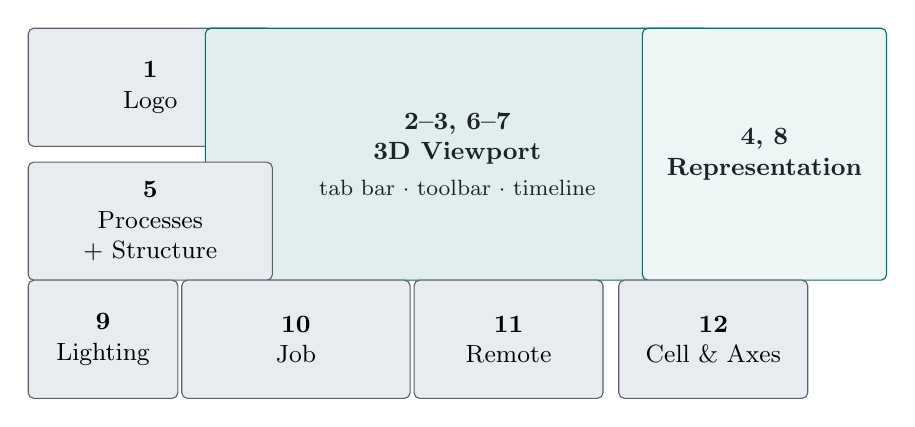
\begin{tikzpicture}[
    zone/.style={draw=shadegray, fill=panelgray, rounded corners=2pt,
                 minimum height=1.5cm, align=center, font=\small},
    view/.style={draw=calangoteal, fill=calangoteal!12, rounded corners=2pt,
                 align=center, font=\small\bfseries, text=calangodark},
    node distance=2mm]
  % row 1
  \node[zone, minimum width=3.1cm] (z1) at (0,3.2) {\textbf{1}\\Logo};
  \node[view, minimum width=6.4cm, minimum height=3.2cm] (v) at (3.9,2.35)
       {\textbf{2--3, 6--7}\\3D Viewport\\[2pt]
        \footnotesize\mdseries tab bar $\cdot$ toolbar $\cdot$ timeline};
  \node[view, minimum width=3.1cm, minimum height=3.2cm, fill=calangoteal!7]
       (z48) at (7.8,2.35) {\textbf{4, 8}\\Representation};
  % row 2
  \node[zone, minimum width=3.1cm] (z5) at (0,1.5) {\textbf{5}\\Processes\\+ Structure};
  % row 3
  \node[zone, minimum width=1.9cm] (z9)  at (-0.6,0) {\textbf{9}\\Lighting};
  \node[zone, minimum width=2.9cm] (z10) at (1.85,0) {\textbf{10}\\Job};
  \node[zone, minimum width=2.4cm] (z11) at (4.55,0) {\textbf{11}\\Remote};
  \node[zone, minimum width=2.4cm] (z12) at (7.15,0) {\textbf{12}\\Cell \& Axes};
\end{tikzpicture}
\end{center}

\begin{description}
  \item[Zone 1 --- branding] The Calango banner. Purely decorative; hide it
    from \menu{View} if you want the vertical space.
  \item[Zone 5 --- \ui{Processes} and \ui{Structure}] The process manager
    (Section~\ref{sec:process-manager}) sits above the structure
    information panel.
  \item[Zones 2--3, 6--7 --- the viewport] The document tab bar, the frame
    toolbar, the 3D canvas, and the playback timeline (visible only for
    trajectories). Covered in Chapter~\ref{ch:viewport}.
  \item[Zones 4 and 8 --- \ui{Representation}] Appearance controls,
    spanning the full height of the right column
    (Chapter~\ref{ch:appearance}).
  \item[Zone 9 --- \ui{Lighting}] Directional light editor.
  \item[Zone 10 --- \ui{Job}] Console and live metric plots for the running
    calculation (Section~\ref{sec:job-panel}).
  \item[Zone 11 --- \ui{Remote Access}] SSH connection, cluster job
    submission and queue monitoring (Chapter~\ref{ch:remote}).
  \item[Zone 12 --- \ui{Unit Cell \& Axes}] Cell wireframe and axes triad
    styling.
\end{description}

\begin{caltip}
Your layout is saved when you quit and restored on the next launch,
including floating panels and window geometry. Every panel has a toggle at
the bottom of the \menu{View} menu, so a panel you closed by accident is
one menu click away.
\end{caltip}

\section{Documents, tabs and the timeline}

Each structure or trajectory you open occupies its own \emph{tab} above the
viewport, and each tab carries its own undo history. All tabs share one
accelerated viewport --- switching tabs changes which document the views
observe, so display settings stay consistent and no OpenGL context is
recreated.

When a document contains more than one frame, the \textbf{playback
timeline} appears below the viewport:

\begin{description}
  \item[Transport buttons] first, previous, play/pause, next, last.
  \item[Scrubber] a tick-marked slider over the frame range.
  \item[Rate] playback speed in frames per second, 0.1--120, default 15.
\end{description}

Trajectories arrive from several places: opening a multi-frame file,
finishing an MD or relaxation run, generating displaced structures in the
phonon builder, or producing a noise ensemble. During a running simulation
the timeline grows in real time as frames stream in
(Section~\ref{sec:live-streaming}).

\section{The Structure panel}
\label{sec:structure-panel}

The \ui{Structure} panel reports what Calango knows about the active
document:

\begin{description}
  \item[\ui{Formula}] Hill-ordered chemical formula.
  \item[\ui{Atoms}, \ui{Bonds}] Counts, with bonds as currently perceived.
  \item[\ui{a, b, c}] Cell vector lengths in \AA{}, to two decimals.
  \item[\ui{$\alpha$, $\beta$, $\gamma$}] Cell angles in degrees.
  \item[\ui{Cell volume}, \ui{Periodic}] Volume and per-axis periodicity.
  \item[\ui{Tolerance}] The spglib symmetry tolerance (\emph{symprec}) used
    for the three fields below, in \AA{}, up to four decimals. Default
    0.001. Raise it for structures with numerical noise --- a relaxed cell
    often needs 0.01 or more before its true symmetry is recognised.
  \item[\ui{Space group}, \ui{Point group}, \ui{Crystal system}] Detected
    symmetry, e.g.\ \texttt{Fd-3m (227)}, \texttt{m-3m}, \texttt{cubic}.
\end{description}

\begin{calwarn}
Symmetry detection needs \texttt{spglib} and a defined unit cell.
\end{calwarn}

\section{Projects and session storage}
\label{sec:projects}

A \emph{project} is one \file{.calproj} file that restores an entire
session: every tab with its structures and trajectory frames, the viewport
colour mapping, and the job console with its recorded metric series.

\begin{description}
  \item[\menu{File}\menusep\menu{Project Workspace}\menusep\menu{Open Project}]
    \kbd{Ctrl}+\kbd{Shift}+\kbd{O}. Replaces the current session, warning
    first if tabs are open.
  \item[\menu{File}\menusep\menu{Project Workspace}\menusep\menu{Save Project}]
    \kbd{Ctrl}+\kbd{S}.
  \item[\menu{File}\menusep\menu{New Workspace}] \kbd{Ctrl}+\kbd{N}. Closes
    everything and starts clean.
\end{description}

Calango tracks unsaved changes. Every undoable edit, tab close and job
launch marks the session dirty; saving or loading a project clears the
flag. Quitting with unsaved changes asks whether to \ui{Save},
\ui{Discard} or \ui{Cancel} --- cancelling (or cancelling the save dialog
that follows) leaves the application open.

\subsection{The managed temporary directory}
\label{sec:calango-tmp}

Simulation jobs and generated ensembles need somewhere to put their working
files. Once a project has been saved, Calango places them in a
\file{.calango\_tmp/} folder \emph{next to the \file{.calproj} file}, one
timestamped subdirectory per task:

\begin{lstlisting}
my_study.calproj
.calango_tmp/
    job_20260721_143255/     run.py, structure.extxyz, md.traj, logs
    noise_20260721_144012/   perturbed.extxyz
    job_20260721_150130/     bands.json, pdos.json
\end{lstlisting}

Until a project has been saved, the same directories are created under the
per-user application data location instead. Either way the process manager
keeps a live link to each one.

\section{The process manager}
\label{sec:process-manager}

The compact \ui{Processes} panel in zone 5 lists every background task of
the session --- local calculations, remote submissions, band-structure
runs, noise ensembles --- with its name, colour-coded status
(\emph{queued}, \emph{running}, \emph{completed}, \emph{failed}) and start
time.

Two buttons act on the selected task:

\begin{description}
  \item[\ui{Open Folder}] Reveals the task's working directory in your file
    manager, for the raw logs and any files Calango does not import.
  \item[\ui{Load Result}] Brings the result back into the workspace.
    Double-clicking the row does the same. Calango inspects the directory
    and opens whatever it finds: band structure and PDOS data open in the
    electronic-structure viewer, trajectories and final geometries open as
    tabs.
\end{description}

The point of keeping these links is that a finished calculation stays one
click from further analysis. A completed MD run can be re-loaded weeks
later and fed to the RDF, distribution or dataset tools without recomputing
anything.

\chapter{The 3D Viewport}
\label{ch:viewport}

The viewport is an OpenGL 3.3 core-profile canvas using instanced rendering
--- one draw call per mesh type --- so structures with tens of thousands of
atoms stay interactive.

\section{Interaction modes}
\label{sec:modes}

What a left-drag does depends on the active \emph{interaction mode}. The
six modes are the first group of buttons on the frame toolbar, each with a
single-letter shortcut:

\begin{center}
\small
\begin{tabular}{@{}llp{8.4cm}@{}}
\toprule
Key & Mode & Left mouse button \\
\midrule
\kbd{R} & Rotation   & Drag orbits the camera around the structure.
                       The default. \\
\kbd{T} & Translation & Drag pans the scene. \\
\kbd{S} & Selection  & Drag draws a rubber-band box and selects every atom
                       inside it. \\
\kbd{I} & Insertion  & Click empty space to add an atom; drag from one atom
                       to another to bond them. \\
\kbd{D} & Distance   & Click two atoms to measure their separation. \\
\kbd{A} & Angle      & Click three atoms (vertex second) to measure the
                       angle. \\
\bottomrule
\end{tabular}
\end{center}

Three gestures work in \emph{every} mode, so navigation never requires
switching back:

\begin{description}
  \item[Middle-drag, or \kbd{Shift}+left-drag] Pan.
  \item[Wheel] Zoom.
  \item[Double-click] Reframe the structure.
\end{description}

The mouse cursor changes with the mode --- an arrow for rotation, an open
hand for panning, a crosshair for selection, insertion and measurement.

\section{Selecting atoms}

A left \emph{click} (no drag) picks the atom under the cursor by ray-cast,
in any mode. \kbd{Ctrl}+click (\kbd{Cmd}+click on macOS) toggles an atom in
or out of the selection, so you can build up a set one atom at a time.
Clicking empty space clears the selection.

In \textbf{Selection} mode a rubber-band drag selects every atom whose
centre falls inside the box; holding \kbd{Ctrl} adds the boxed atoms to the
existing selection instead of replacing it. With the viewport focused,
\kbd{Delete} or \kbd{Backspace} removes the selected atoms and the bond
network is rebuilt immediately.

The status bar reports the selection size, and several tools act on it: the
bond-order buttons need exactly two atoms, the bond editor can pull a pair
straight from the selection, and \menu{Edit}\menusep\menu{Selection} can
change the element of, or translate, whatever is selected.

\section{Measuring distances and angles}
\label{sec:measure}

Measurement modes accumulate clicks on atoms and draw the result directly
on the canvas --- markers on the chosen atoms, dashed connecting lines, and
the value in a floating label. The same value is written to the status bar,
for example:

\begin{lstlisting}
Distance Si(0) - Si(4): 2.351 A
Angle O(2) - Si(0) - O(5): 109.47 deg
\end{lstlisting}

\begin{description}
  \item[Distance] Two atoms; result in \AA{} to three decimals.
  \item[Angle] Three atoms; the \emph{second} atom clicked is the vertex.
    Result in degrees to two decimals.
\end{description}

Clicking empty space clears the current measurement, and clicking again
after a completed one starts fresh. Dragging still orbits the camera, so
you can rotate the structure between clicks to reach an atom hidden behind
another. Measurements are cleared automatically when you switch modes or
load a different structure.

\section{Fixed-angle rotations}

The toolbar's rotation cluster turns the scene by exact increments about
the world axes --- useful for reproducible figure orientations.

\begin{description}
  \item[Angle step] An editable spin box, 1--180\textdegree, default
    15\textdegree.
  \item[\ui{X+} \ui{X$-$} \ui{Y+} \ui{Y$-$} \ui{Z+} \ui{Z$-$}]
    Counter-clockwise and clockwise rotation about each axis by exactly
    that step.
\end{description}

Each click animates smoothly over about 200\,ms, and rapid clicks compose
exactly: four presses of \ui{Z+} at 90\textdegree{} return the scene to
where it started. The axes triad follows the rotation, and picking,
selection and measurements all stay consistent with what you see.

\section{Framing, alignment and projection}

\begin{description}
  \item[\kbd{F}] Frame the structure: centre it and back the camera off far
    enough to see all of it. Also on the toolbar and in
    \menu{View}\menusep\menu{Alignment}.
  \item[Align with XY / XZ / YZ] Look straight down the remaining
    Cartesian axis. Toolbar buttons, or
    \menu{View}\menusep\menu{Alignment}. Alignment clears any accumulated
    fixed-angle rotation, so the result is a true axis-aligned view.
  \item[\kbd{O}] Toggle orthographic versus perspective projection. The
    orthographic frustum is matched to the perspective field of view at the
    camera's target distance, so the structure keeps its apparent size
    across the switch --- and zoom keeps working in both.
\end{description}

\begin{caltip}
Orthographic projection is what you want for figures where lattice
directions must read as parallel: perspective foreshortening makes a
supercell look subtly sheared.
\end{caltip}

\section{Inserting atoms and bonds}

In \textbf{Insertion} mode (\kbd{I}) the toolbar's element button --- which
shows the active symbol, \texttt{C} by default --- selects what gets
placed. Click it to choose any element from the graphical periodic table.

\begin{description}
  \item[Click on empty space] Inserts one atom of the active element there.
    The atom lands on the plane through the camera's target point facing
    the viewer, so what you click is where it appears.
  \item[Drag from one atom to another] Creates a bond between them, added
    as a manual bond override.
  \item[Click on an existing atom] Selects it, as in any other mode.
\end{description}

Both operations are single undo steps.

\begin{calnote}
Because inserted atoms land on the camera-target plane, the depth of a new
atom depends on the current view. Place atoms from an aligned, orthographic
view when the exact coordinate matters, or insert roughly and then set
exact coordinates with \menu{Edit}\menusep\menu{Add Atom}, which takes
numeric $x$, $y$, $z$.
\end{calnote}

\section{Visual effects}
\label{sec:visual-effects}

\menu{View}\menusep\menu{Visual Effects} toggles the \ui{Visual Effects}
dock --- the scene stays interactive while you tune it. It is a five-tab
panel running from what lights the scene, through the scene itself, to the
passes that post-process the finished image: \ui{Light} (the studio
lighting rig, Chapter~\ref{ch:appearance}), \ui{Shadow}, \ui{Fog},
\ui{Blur} and \ui{SSAO}. Every effect defaults to off. The ground plane
used to sit here as a \ui{Floor} tab; it now lives in the \ui{Spatial
References} dock instead (Chapter~\ref{ch:appearance}), since it draws a
whole extra object into the scene rather than an image filter.

\subsection{Shadows}

Real-time shadow mapping with percentage-closer filtering: atoms and bonds
cast shadows onto neighbouring geometry, including the floor when it is on.
Off by default; adds roughly one extra depth-only pass per frame.

\begin{description}
  \item[\ui{Intensity}] 0.00--1.00. How much direct light an occluded
    surface loses --- ambient light is never attenuated, so even at 1.00
    shadowed geometry stays readable rather than going black.
  \item[\ui{Softness / blur radius}] 0--6 texels. The PCF blur radius: 0
    gives hard, aliased edges; each step averages a wider neighbourhood, so
    quality and cost both rise together. 2--3 suits most structures.
\end{description}

The shadow projection follows the \textbf{primary light} --- the first
entry under the \ui{Light} tab. Re-aiming that light re-aims the shadows;
fill lights stay unshadowed, which is what keeps occluded regions legible.

\subsection{Distance fog}

Fades distant geometry into the background colour, which makes the depth
ordering of a thick slab or a large nanoparticle immediately readable.

\begin{description}
  \item[\ui{Mode}] \ui{Linear (start $\rightarrow$ end)} fades uniformly
    between two distances; \ui{Exponential (density)} follows
    $e^{-\rho d}$.
  \item[\ui{Start distance}, \ui{End distance}] The linear ramp, in \AA{}.
    Defaults 15 and 80.
  \item[\ui{Density}] The exponential coefficient, default 0.03.
\end{description}

The fog colour tracks the viewport background automatically, so geometry
always fades into whatever backdrop you have chosen.

\subsection{Depth of field}

A post-processing pass that blurs geometry away from the focal plane, in
proportion to its circle of confusion.

\begin{description}
  \item[\ui{Blur strength}] Maximum blur radius in pixels, 1--20.
  \item[\ui{Focus range}] The depth band that stays sharp, in \AA{}.
  \item[\ui{Focus offset}] Shifts the focal plane relative to the camera
    target, in \AA{}.
\end{description}

\begin{calnote}
Depth of field renders the scene into an offscreen buffer before
compositing, which means multisample anti-aliasing is unavailable while it
is enabled. For final figures, decide which of the two matters more ---
crisp edges or the depth cue.
\end{calnote}

\chapter{Getting Data In and Out}
\label{ch:data}

\section{Supported formats}
\label{sec:formats}

All structure I/O goes through \texttt{ase.io}, so Calango reads and writes
every format ASE knows. The file dialog offers the common ones directly:

\begin{center}
\small
\begin{tabular}{@{}lp{9.2cm}@{}}
\toprule
Family & Extensions \\
\midrule
XYZ            & \file{.xyz}, \file{.extxyz} \\
Crystallography& \file{.cif} \\
VASP           & \file{POSCAR}, \file{CONTCAR}, \file{.vasp} \\
ASE            & \file{.traj} \\
Quantum ESPRESSO & \file{.in}, \file{.pwi}, \file{.pwo}, \file{.out} \\
CASTEP         & \file{.cell} \\
LAMMPS         & \file{.data}, \file{.dump}, \file{.lammpstrj} \\
Gaussian       & \file{.gjf}, \file{.com} \\
SHELX          & \file{.res} \\
\bottomrule
\end{tabular}
\end{center}

\begin{calnote}
Extended-XYZ per-atom arrays are imported as \emph{scalar fields} and
\emph{vector fields}. A \texttt{charges} or \texttt{forces} column becomes
selectable in the \ui{Custom property} colour mode, and \texttt{forces} or
\texttt{momenta} enable the force and velocity arrow overlays. This is the
simplest route for visualising per-atom data computed elsewhere: write it
as an extxyz column and open the file.
\end{calnote}

\section{Opening structures and trajectories}

\begin{description}
  \item[\menu{File}\menusep\menu{Open}\menusep\menu{Structure}]
    \kbd{Ctrl}+\kbd{O}.
  \item[\menu{File}\menusep\menu{Open}\menusep\menu{Trajectory}]
    \kbd{Ctrl}+\kbd{T}.
\end{description}

Both entries read \emph{every} frame in the file. A single-frame file opens
as a plain structure tab; a multi-frame file opens as a trajectory with the
timeline active. In practice the two entries differ only in the file
filter, so either works for either kind of file.

Opening a \file{.calproj} file --- from the command line, your file
manager, or the structure dialog --- restores the saved session rather than
loading a geometry.

\section{Saving structures and trajectories}

\begin{description}
  \item[\menu{File}\menusep\menu{Save}\menusep\menu{Structure As}]
    \kbd{Ctrl}+\kbd{Shift}+\kbd{S}. Writes the currently displayed frame.
    The name is suggested from the document's own, with the default
    extension; the format follows the filter you pick, and a name typed
    without an extension is given the filter's own.
  \item[\menu{File}\menusep\menu{Save}\menusep\menu{Trajectory As}]
    \kbd{Ctrl}+\kbd{Shift}+\kbd{T}. Writes all frames of the active
    document as extended XYZ, multi-frame XYZ, ASE \file{.traj}, or
    multi-model PDB.
\end{description}

\begin{calnote}
\textbf{Extended XYZ is the default everywhere.} It is pre-selected in every
open and save dialog in the application --- structures, trajectories, NEB
endpoints, dataset imports --- and it is what \menu{Save Structure As}
writes unless you choose otherwise. The reason is that it is the only format
in the list that round-trips everything a Calango document carries: cell and
periodicity, per-atom magnetic moments and charges, forces and velocities,
and arbitrary extra columns. Plain \file{.xyz} silently drops the cell; CIF
drops the calculator results; POSCAR drops nearly everything but the
positions.

Every other format is still one entry down in the same list, so nothing has
become harder to reach --- only the \emph{default} changed, to the format
that loses nothing.
\end{calnote}

\section{The database and preset browser}
\label{sec:database}

\menu{Build}\menusep\menu{From Database} opens a two-tab browser.

\subsection{Presets}

Seven benchmark structures ship with Calango, each annotated with a
suggested calculator:

\begin{center}
\small
\begin{tabular}{@{}lll@{}}
\toprule
Preset & File & Suggested calculator \\
\midrule
Diamond (bulk C)       & \file{diamond.vasp}            & MACE-MP-0 \\
MoS$_2$ 2H (bulk)      & \file{mos2\_2h\_bulk.vasp}     & MACE-MP-0 \\
Graphene monolayer     & \file{graphene.vasp}           & MACE-MP-0 \\
MoS$_2$ 1H (monolayer) & \file{mos2\_1h\_monolayer.vasp}& MACE-MP-0 \\
Benzene                & \file{benzene.xyz}             & MACE-OFF (or EMT) \\
Naphthalene            & \file{naphthalene.xyz}         & MACE-OFF \\
Coronene               & \file{coronene.xyz}            & MACE-OFF \\
\bottomrule
\end{tabular}
\end{center}

Select a row and press \ui{Load Selected}, or double-click it.

\subsection{Materials Project}

The second tab fetches structures by Materials Project ID.

\begin{description}
  \item[\ui{API key}] Masked field, pre-filled from your saved setting or
    from \opt{MP\_API\_KEY} in the environment. It is stored as you type.
  \item[\ui{Material ID}] For example \texttt{mp-149} (silicon). Pressing
    \kbd{Enter} triggers the fetch.
  \item[\ui{.env file}] Shows the current environment file path, with
    \ui{Browse\ldots} to point elsewhere and \ui{Reload} to re-import the
    key (Section~\ref{sec:envfile}).
  \item[\ui{Fetch Structure}] Downloads the entry and opens it in a new
    tab, reporting the formula and atom count.
\end{description}

\begin{calwarn}
Needs a network connection and a personal API key from
\url{https://materialsproject.org/api}.
\end{calwarn}

\chapter{Building Structures}
\label{ch:building}

Everything in the \menu{Build} menu produces a new structure, either
replacing the active one or opening in a new tab. All of it runs through
ASE, so a working Python environment is a prerequisite throughout this
chapter.

\section{Supercells}

\menu{Edit}\menusep\menu{Unit Cell}\menusep\menu{Create Supercell} repeats
the active structure along its lattice vectors. Three spin boxes,
\ui{Repeat along a/b/c}, each 1--20, default $2 \times 1 \times 1$. The
operation is undoable and requires a defined cell along every repeated
direction.

\section{The surface slab wizard}
\label{sec:slab-wizard}

\menu{Build}\menusep\menu{Surface Slab} cleaves a slab from the active bulk
structure in three guided stages. Unlike a plain Miller-index dialog, each
stage shows you the consequence of your choice before you commit.

\subsection{Stage 1 --- surface orientation}

Set the Miller indices $(h\,k\,l)$ with three spin boxes ($-9$ to $9$), or
work the other way round: drag the red \textbf{u} and green \textbf{v}
handles on the interactive lattice canvas to any two lattice points, and
Calango computes the nearest integer $(h\,k\,l)$ for the plane they span.
The header shows the current vectors and resulting indices live, and the
info line reports $|u|$, $|v|$ and the angle between them.

Rotate the axonometric view by dragging; only non-collinear handle pairs
are accepted. \ui{Next} unlocks once a test cut succeeds --- $(0\,0\,0)$ is
rejected as not a plane.

\subsection{Stage 2 --- cut, thickness and terminations}

Calango builds a reference stack of eight bulk repeats and clusters the
atoms into atomic layers (0.10\,\AA{} tolerance). The cross-section canvas
draws each layer as a dashed line labelled with its $z$ coordinate, with
the current selection band highlighted between an orange \emph{top
termination} and a teal \emph{bottom termination}.

\begin{description}
  \item[Click a layer] Moves whichever boundary is nearer the click, so you
    can set either termination directly.
  \item[\ui{Layers in slab}] Sets the count numerically.
  \item[\ui{Thickness}] The same choice in \AA{}; it snaps to whole atomic
    layers above the bottom termination.
\end{description}

The info line reads back the selection, for example \emph{layers 1--8 of
16 (8 layers, 12.45\,\AA)}.

\subsection{Stage 3 --- vacuum and preview}

\ui{Top vacuum} and \ui{Bottom vacuum} (0--80\,\AA{}, default 10 each) pad
the cell along the surface normal. \ui{Symmetric vacuum (centered slab)},
checked by default, mirrors the top value to the bottom. A live 3D preview
shows the finished slab, with atom count, slab thickness and total cell
height. \ui{Finish} inserts it as a new tab labelled, for example,
\emph{(1 1 1) slab, 8 layers}.

\section{Liquid and gas interfaces}
\label{sec:liquid-interface}

\menu{Build}\menusep\menu{Liquid / Gas Interface} opens a fluid region on the
structure in the current tab and packs it with a liquid, a gas, a mixture, or
an ionic solution --- the solid/liquid and solid/gas cells that electro\-chem\-istry,
catalysis and adsorption studies start from. It consumes a structure rather
than generating one, so build or open the substrate first; a surface slab
from \S\ref{sec:slab-wizard} is the usual input. The result opens as a new
tab and the substrate's own tab is left untouched.

\subsection{Stage 1 --- geometry and region}

\begin{description}
  \item[\ui{Interface direction}] Which lattice vector the region is opened
    along; \emph{c} for a slab built by this application. The region is
    bounded by planes normal to the \emph{other} two lattice vectors, so it
    stays commensurate with the cell even when that cell is tilted.
  \item[\ui{Region thickness}] The gap between the top face of the structure
    and the bottom face of its own periodic image. The cell is grown --- or
    shrunk --- to make this \emph{exact}, whatever vacuum the input already
    carried. Asking for 20\,\AA{} of water and silently getting 20\,\AA{}
    plus the slab's existing 15\,\AA{} is the usual way to end up with an
    accidentally dilute interface.
  \item[\ui{Lateral supercell}] Repeats the substrate in the two directions
    that lie \emph{in} the interface plane, before the region is opened. A
    wider cell is usually what a solvation study needs: the fluid's
    correlation length is several \AA{}, and a $1\times1$ surface cell forces
    it to be periodic on a shorter length than that.
  \item[\ui{Surface clearance}] Closest approach between any fluid atom and
    any substrate atom (default 2.2\,\AA{}).
  \item[\ui{Move the substrate to the bottom of the cell}] On by default, so
    the fluid region is one contiguous block. Turn it off when the slab was
    positioned deliberately --- a symmetric slab centred in its cell, for
    instance.
\end{description}

The summary underneath reports the cell before and after, the fillable
volume, and how many water molecules that volume holds at ambient density.

\subsection{Stage 2 --- solvation and mixture}

\ui{Liquid / gas mixture} is a table of species and mole fractions. The
fractions are normalised, so $\{3\ \text{water},\ 1\ \text{ammonia}\}$ and
$\{0.75,\ 0.25\}$ request the same mixture. \ui{Amount} chooses between a
target mass density and an explicit molecule count.

\ui{Ionic species} inserts salts or bare ions by \emph{formula unit}. A salt
expands into its ions, so three units of (NH$_4$)$_2$SO$_4$ is six ammonium
and three sulfate and the cell stays neutral by construction. Bare ions are
offered too, for the cases where an unbalanced charge is deliberate; the net
charge is reported below the table, in orange when it is not zero.

Ions are placed \emph{before} the solvent and their mass counts against the
density target. Both matter: a packing that saturated could otherwise drop an
ion and silently change the stoichiometry, and a density target that ignored
the ions would give a brine at the density of water with salt added on top of
it.

\begin{caltip}
A gas at its 1\,bar density comes to a fraction of a molecule in a cell of
interface size, so picking a gas switches the page to an explicit molecule
count. That is the physically meaningful control: in a periodic cell the
molecule count \emph{is} the partial pressure.
\end{caltip}

\subsection{What the packer does, and what it does not}

Molecules are proposed at random positions with uniformly random
orientations and kept when they clear everything already placed. Two fluid
molecules are excluded on their centres, using a tabulated effective radius
per species, with an atom-level floor on top so that two molecules facing
each other cannot interlock their hydrogens; the substrate is checked atom by
atom, because that surface is fixed and a molecule started inside it cannot
relax out. The packing is seeded and therefore reproducible.

\begin{calwarn}
The result is a legitimate \emph{starting point} --- right composition, right
density, no overlaps --- and it is not an equilibrated liquid. A random
packing has no hydrogen-bond network and a potential energy far above the
equilibrium one. Quoting a diffusion coefficient, an interface energy or a
work of adhesion computed directly on this cell would be reporting a property
of the random number generator. Equilibrate with molecular dynamics
(\S\ref{sec:md}) first.
\end{calwarn}

Random sequential packing saturates below the equilibrium density of a
hydrogen-bonded liquid; around 90\% of the target is typical for water and is
perfectly usable. A larger shortfall is reported explicitly after the cell
opens, together with what to do about it.

\begin{calnote}
The species library holds only molecules whose geometry is fixed by symmetry
plus a bond length and, where needed, one angle: water, ammonia, HF, H$_2$S,
the common diatomic and small polyatomic gases, the noble gases, the alkali
and alkaline-earth cations, the halides, and the molecular ions
NH$_4^{+}$, H$_3$O$^{+}$, OH$^{-}$, NO$_3^{-}$, CO$_3^{2-}$, SO$_4^{2-}$ and
PO$_4^{3-}$. Species that need a real optimised geometry --- the alcohols,
anything with a torsional degree of freedom --- are deliberately absent
rather than approximated: a molecule with plausible-looking but wrong
internal coordinates produces a cell that nobody notices is wrong until the
first relaxation step tears it apart.
\end{calnote}

\section{Nanomaterials}

\menu{Build}\menusep\menu{Nanomaterial Builder} generates four families of
low-dimensional carbon and TMD structures. Pick the type at the top; the
form below changes to match.

\begin{description}
  \item[Graphene sheet] Lattice constant $a$ (default 2.46\,\AA), repeats
    $n_x \times n_y$ (default $4 \times 4$), vacuum (default 10\,\AA).
  \item[Graphene nanoribbon] Width and length in unit cells (default 6 each),
    \ui{Edge type} \ui{Zigzag} or \ui{Armchair}, and
    \ui{Hydrogen-terminate edges} (on by default).
  \item[Carbon nanotube] Chiral indices $n$ and $m$ (default 6, 6), length
    in unit cells, C--C bond length (default 1.42\,\AA), vacuum (default
    8\,\AA). $(0,0)$ is rejected.
  \item[TMD monolayer (MX$_2$)] An editable formula combo --- \texttt{MoS2},
    \texttt{MoSe2}, \texttt{WS2}, \texttt{WSe2}, \texttt{MoTe2},
    \texttt{NbSe2}, or anything else you type --- \ui{Phase} \texttt{2H} or
    \texttt{1T}, lattice constant (default 3.16\,\AA), X--X thickness
    (default 3.19\,\AA), repeats and vacuum.
\end{description}

\section{Metallic nanoparticles}
\label{sec:nanoparticle}

\menu{Build}\menusep\menu{Metallic Nanoparticle (Wulff)} builds clusters
two ways. Choose the element from the periodic table, then a mode.

\subsection{Wulff construction}

The equilibrium shape of a crystal is the one minimising total surface
energy at fixed volume; the Wulff construction produces it from the
relative surface energies of the exposed facets.

\begin{description}
  \item[Facet table] One row per facet: $h$, $k$, $l$ and
    $\gamma$ (relative surface energy). Defaults are $(111)\!=\!1.0$,
    $(100)\!=\!1.1$, $(110)\!=\!1.2$. \ui{Add Facet} and
    \ui{Remove Selected} edit the list.
  \item[\ui{Target atoms}] The requested size, default 200. The
    construction lands on the nearest achievable closed shape.
  \item[\ui{Size rounding}] \texttt{closest}, \texttt{above} or
    \texttt{below}.
  \item[\ui{Lattice}] \texttt{fcc}, \texttt{bcc} or \texttt{sc}.
\end{description}

Only the \emph{ratios} of the $\gamma$ values matter. Lowering
$\gamma(111)$ relative to $\gamma(100)$ grows the $(111)$ facets and drives
an fcc metal from a cube towards a truncated octahedron.

\subsection{Spherical cluster}

Carves every atom within a cutoff radius of the centre out of a bulk
lattice --- \texttt{fcc}, \texttt{bcc}, \texttt{sc} or \texttt{hcp}. Set
\ui{Radius} (default 10\,\AA). Useful when you want a specific diameter
rather than a thermodynamic shape.

Both modes centre the cluster with 6\,\AA{} of vacuum and clear periodicity.
\ui{Lattice constant} may be left at \ui{ASE default} to use the tabulated
value for the element.

\section{Special quasirandom structures}
\label{sec:sqs}

\menu{Build}\menusep\menu{Special Quasirandom Structure (SQS)} builds a
substitutional alloy whose short-range order approximates a truly random
solid solution --- the standard way to model a disordered alloy in a small
periodic cell.

\begin{description}
  \item[\ui{Supercell}] Repetitions $n_1 \times n_2 \times n_3$, default
    $2 \times 2 \times 2$.
  \item[\ui{Replace element}] Whose sites form the alloy sublattice.
  \item[\ui{Composition}] Target occupancies as symbol:fraction pairs, e.g.
    \texttt{Cu:0.75, Au:0.25}. Fractions are normalised and rounded to
    whole atoms by largest remainder.
  \item[\ui{First shell cutoff}, \ui{Second shell cutoff}] The pair shells
    whose Warren-Cowley parameters are driven toward zero. Defaults 3.2 and
    4.8\,\AA; set the second to \ui{off} to use one shell.
  \item[\ui{MC steps}, \ui{Random seed}] Anneal length and reproducibility.
\end{description}

If \texttt{icet} is importable, Calango uses its \texttt{generate\_sqs};
otherwise it falls back to a built-in simulated annealer that minimises
$\sum \alpha^2$ over the chosen shells using only NumPy and ASE neighbour
lists. The resulting tab is labelled with the backend that produced it, and
the internal backend also reports its residual objective --- a value near
zero means the decoration is essentially ideal.

\begin{caltip}
Verify the result with \menu{Analysis}\menusep\menu{Warren-Cowley analysis}
(Section~\ref{sec:warren-cowley}): a good SQS shows $\alpha \approx 0$ for
the shells you optimised.
\end{caltip}

\section{Normal modes and phonons}
\label{sec:phonon-builder}

\menu{Build}\menusep\menu{Normal Modes / Phonon Builder} sets up a
finite-displacement vibrational calculation. Calango detects whether the
structure is periodic and adapts:

\begin{description}
  \item[Periodic] Supercell finite displacements via \texttt{ase.phonons},
    giving dispersion and DOS.
  \item[Isolated molecule] $\Gamma$-point normal modes via
    \texttt{ase.vibrations}, giving frequencies and per-mode animation
    trajectories that Calango opens directly.
\end{description}

\subsection{Parameters}

\begin{description}
  \item[\ui{Mode}] \ui{Run vibrational calculation}, or
    \ui{Generate displaced structures only (new tab)} to export the
    displacement set for an external DFT code.
  \item[\ui{Supercell (a $\times$ b $\times$ c)}] Default $2\times2\times2$,
    periodic structures only.
  \item[\ui{Displacement $\delta$}] Default 0.01\,\AA.
  \item[\ui{Displaced structures}] A read-only count: $6N+1$ for $N$
    supercell atoms.
  \item[\ui{Calculator}] EMT, Lennard-Jones or MACE --- deliberately
    limited to calculators needing no external binary or pseudopotentials.
  \item[\ui{Band-path points}, \ui{DOS k-grid}] Sampling for the dispersion
    and the phonon density of states (defaults 100 and 20).
\end{description}

Like the calculator dialog, the generated ASE script is shown in an
editable pane and can be saved with \ui{Save Script\ldots}.

Outputs are $\Gamma$-point frequencies in the job console, plus
\file{phonon\_bands.csv} and \file{phonon\_dos.csv} in the job directory.

\begin{calnote}
Displacements are applied to every atom of the expanded supercell
($6N_\text{supercell}+1$ configurations), following the standard
finite-displacement recipe without symmetry reduction. For large
supercells this is the dominant cost; symmetry-reduced displacement sets
are a planned improvement.
\end{calnote}

\section{Structure perturbation and noise}
\label{sec:noise}

\menu{Build}\menusep\menu{Structure Perturbation / Noise} adds random
displacements --- for shaking a structure out of a symmetric saddle point,
or for generating training ensembles for machine-learning potentials.

\begin{description}
  \item[\ui{Distribution}] \ui{Gaussian (normal)} or \ui{Uniform}.
  \item[\ui{Amplitude}] Default 0.05\,\AA. For Gaussian this is $\sigma$
    per component; for uniform it is the half-width.
  \item[\ui{Random seed}] Default 42, for reproducibility.
  \item[\ui{Perturb atomic positions}] On by default.
  \item[\ui{Perturb unit cell vectors (random strain)}] Atoms follow the
    cell affinely, preserving fractional coordinates.
  \item[\ui{Frames}] 1 perturbs in place; more generates a trajectory.
  \item[\ui{Accumulation}] \ui{Independent} draws each frame from the
    original structure; \ui{Cumulative} performs a random walk from the
    previous frame.
\end{description}

A multi-frame run opens as a trajectory whose frame 0 is the unperturbed
original, is registered in the process manager, and is checkpointed to
\file{perturbed.extxyz} in the managed temporary directory
(Section~\ref{sec:calango-tmp}) --- so the ensemble can be reloaded later
and fed to the analysis or dataset tools.

\chapter{Editing Structures}
\label{ch:editing}

Every operation in this chapter is a single undo step.
\menu{Edit}\menusep\menu{Undo} (\kbd{Ctrl}+\kbd{Z}) and
\menu{Edit}\menusep\menu{Redo} (\kbd{Ctrl}+\kbd{Shift}+\kbd{Z}) walk a
per-document history up to 50 states deep.

\section{Atoms}

\begin{description}
  \item[\menu{Edit}\menusep\menu{Add Atom}] \kbd{Ctrl}+\kbd{Shift}+\kbd{A}.
    Choose the element from the graphical periodic table and type exact
    $x$, $y$, $z$ coordinates. For placing atoms by eye instead, use
    Insertion mode in the viewport (\kbd{I}).
  \item[\menu{Edit}\menusep\menu{Selection}\menusep\menu{Change Element of Selection}]
    Replaces the species of every selected atom, again via the periodic
    table.
  \item[\menu{Edit}\menusep\menu{Selection}\menusep\menu{Translate Selection}]
    Shifts the selection by a $\Delta x$, $\Delta y$, $\Delta z$ vector in
    \AA.
  \item[\menu{Edit}\menusep\menu{Delete Selected Atoms}] \kbd{Delete}.
    Removes the selection; with the viewport focused in Selection mode,
    \kbd{Backspace} does the same.
\end{description}

Deleting atoms re-indexes everything that referenced them --- bond
overrides, bond orders and per-atom fields all follow correctly.

\section{The periodic table selector}

Wherever an element must be chosen, Calango opens a graphical periodic
table: $Z = 1$ to 118 in the standard 18-group layout, f-block below,
coloured by chemical family. One click selects and closes.

\section{Bond perception}
\label{sec:bonds}

By default Calango perceives bonds by distance: atoms $i$ and $j$ are
bonded when
\[
  d_{ij} < t \cdot \bigl(r_\text{cov}(i) + r_\text{cov}(j)\bigr),
\]
with covalent radii from Cordero \emph{et al.} and a tolerance $t$ you
control. With a periodic cell the minimum-image convention applies, so
bonds across cell boundaries are found and drawn correctly.

\menu{Edit}\menusep\menu{Bond Editor} (\kbd{Ctrl}+\kbd{B}) exposes both the
automatic rule and manual overrides:

\begin{description}
  \item[\ui{Automatic bond detection}] Turn it off to draw \emph{only}
    manually added bonds --- the right choice for coarse-grained or
    schematic figures.
  \item[\ui{Covalent cutoff multiplier}] The tolerance $t$, 0.50--2.50,
    default 1.15. Applied live, so you can dial it until the picture is
    right.
  \item[\ui{Manual Bonds}] Two 1-based atom-index spin boxes, or
    \ui{From Selection} to fill them from a two-atom viewport selection.
    The info line shows the current pair's distance next to the automatic
    cutoff for that pair, which makes it obvious whether a bond is
    borderline.
  \item[\ui{Add Bond}] Forces a bond regardless of distance.
  \item[\ui{Suppress Bond}] Removes an automatically perceived bond.
  \item[\ui{Active overrides}] Lists every override as \emph{added} or
    \emph{suppressed}, with the pair and its distance.
    \ui{Clear Override} and \ui{Clear All} undo them.
\end{description}

Overrides live on the structure and are saved in the project file.

\section{Bond orders}
\label{sec:bond-orders}

Calango never guesses multiple bonds. Every perceived bond starts as a
single bond, and orders are assigned deliberately --- distance-based
perception of double and triple bonds is unreliable, particularly for
inorganic and metallic systems where short contacts are common.

To assign one, select exactly two atoms in the viewport
(\kbd{Ctrl}+click the second) and use the \ui{Bond order} buttons in the
\ui{Representation} panel: \ui{Single}, \ui{Double}, \ui{Triple}. The
buttons are disabled until a pair is selected.

An order of two or three renders as that many parallel cylinders, and also
forces the bond to exist even if the pair lies outside the automatic
cutoff. Orders persist in project files.

\begin{calnote}
A consequence worth knowing: molecules like benzene or CO$_2$ render with
all-single bonds when first opened. Assign the orders you want to display;
they are a presentation property, not an input to any calculation.
\end{calnote}

\chapter{Appearance and Representation}
\label{ch:appearance}

\section{The Representation panel}

\subsection{Representation mode}

\ui{Mode} selects how atoms and bonds are drawn:

\begin{description}
  \item[\ui{Ball-and-Stick}] Spheres at a fraction of the covalent radius,
    bonds as cylinders. The default.
  \item[\ui{Space-filling (CPK)}] Spheres at approximately the van der
    Waals radius; bonds are hidden inside the atoms.
  \item[\ui{Wireframe}] Bonds only, drawn as lines with points at the atom
    positions --- the cheapest mode for very large systems.
\end{description}

\ui{Atom radius} and \ui{Bond width} scale everything globally, 0.20--3.00,
each with a slider and a synchronised spin box for exact values.

\subsection{Colouring atoms}
\label{sec:color-modes}

\ui{Color by} offers four mappings, applied consistently to atoms and to
their halves of each bond:

\begin{description}
  \item[\ui{Element (CPK)}] The Jmol palette, with per-element overrides.
  \item[\ui{Coordination number (CN)}] Discrete coordination numbers on a
    gradient.
  \item[\ui{Generalized CN (GCN)}] Continuous generalised coordination
    numbers --- excellent for distinguishing terraces, steps, edges and
    vertices on nanoparticles and slabs.
  \item[\ui{Custom property}] Any per-atom scalar field the structure
    carries: charges, force magnitudes, extended-XYZ columns, or a computed
    field such as \texttt{local\_entropy}. \ui{Property} selects which.
\end{description}

For the three scalar modes, \ui{Gradient} chooses the colour map ---
\ui{Viridis}, \ui{Plasma}, \ui{Turbo}, \ui{Inferno}, \ui{Magma},
\ui{Cividis}, \ui{Hot}, \ui{Afmhot}, \ui{Coolwarm}, \ui{Rainbow} --- and
\ui{Invert palette} reverses the scalar-to-colour mapping, matching
matplotlib's \texttt{\_r} variants. \ui{Range} reads back the min and max
of the active field, so the legend is never ambiguous.

\begin{caltip}
Viridis and Cividis are perceptually uniform and colour-vision safe;
Coolwarm is the right choice for signed quantities such as charges or
potentials, where the zero point should read as neutral. Rainbow is
included because reviewers sometimes ask for it, not because it is a good
default.
\end{caltip}

Colour mapping is recomputed for every frame during trajectory playback, so
CN, GCN and property maps stay live throughout an animation.

\subsection{Bonds and vectors}

\begin{description}
  \item[\ui{Gradient bond coloring}] Blends each bond smoothly from one
    atom's colour to the other's, instead of the classic half-and-half
    split.
  \item[\ui{Force vectors}, \ui{Velocity vectors}] Draw per-atom vectors as
    lit 3D arrows. Each is enabled only when the structure actually carries
    that field; the tooltip explains what is missing when it does not.
  \item[\ui{Vector scale}] Arrow length in \AA{} per field unit,
    0.05--200, default 10.
\end{description}

\subsection{Per-element styling}

\ui{Element Settings\ldots} opens a table of the elements present in the
structure. Each row offers a colour swatch and a radius scale
(10--300\,\%, where exactly 100\,\% means "no override"), plus a
\ui{Reset} button. \ui{Reset All} clears every override at once.

\ui{Background} sets the viewport background colour. Distance fog, if
enabled, automatically fades into whatever you choose.

\section{Unit cell and axes}

The \ui{Unit Cell \& Axes} panel (zone 12):

\begin{description}
  \item[\ui{Show unit cell}] Also on \menu{View}\menusep\menu{Overlays}.
  \item[\ui{Cell color}] Wireframe colour.
  \item[\ui{Cell line width}] 1.0--8.0, default 2.0. A width of 1 draws
    plain GL lines; anything larger renders the edges as lit tubes.
  \item[\ui{Show axes triad}] The corner orientation indicator.
  \item[\ui{Axes style}] \ui{Cartesian (X, Y, Z)} or
    \ui{Lattice vectors (a1, a2, a3)}.
  \item[\ui{Axes size}] On-screen size of the triad, 48--240\,px.
\end{description}

\begin{calnote}
Core-profile OpenGL clamps hardware line width to one pixel, which is why
thick cell edges are drawn as tube geometry rather than wide lines. The
tubes are lit like the rest of the scene, so they also read correctly in
ray-traced exports.
\end{calnote}

\section{Lighting}

The \ui{Light} tab of the \ui{Visual Effects} panel (zone 9) edits up to
four directional lights with
Blinn-Phong shading. The default studio setup is three lights: a warm key
carrying the speculars, a cooler fill from the opposite side, and a back
(rim) light that separates atom silhouettes from the background.

Select a light in the list, then edit:

\begin{description}
  \item[\ui{Direction (view space)}] Three components, $-5$ to $5$. Because
    directions are in view space, the lighting stays fixed relative to the
    viewer as you orbit --- the structure turns, the studio does not.
  \item[\ui{Ambient}, \ui{Diffuse}, \ui{Specular}] Per-light colours.
\end{description}

\ui{Add} appends a fill light from the opposite side; \ui{Remove} deletes
the selected one. At least one light always remains.

\chapter{Running Simulations}
\label{ch:simulations}

\section{The calculation dialog}

\menu{Simulation}\menusep\menu{New Calculation (ASE)} (\kbd{Ctrl}+\kbd{R})
is the main entry point. The left half is a form; the right half is the ASE
script that form produces, live and editable.

\subsection{Calculators}

\begin{center}
\small
\begin{tabular}{@{}lp{8.4cm}@{}}
\toprule
Calculator & Notes \\
\midrule
EMT             & Effective medium theory. Fast, ships with ASE, useful for
                  testing a workflow before committing compute. \\
Lennard-Jones   & Ships with ASE. \\
Quantum ESPRESSO& DFT; needs \texttt{pw.x} and pseudopotentials. \\
VASP            & DFT; needs a license and POTCARs. \\
MACE            & Machine-learning potential; needs \texttt{mace-torch}. \\
GPAW            & DFT as a Python package. \\
SIESTA          & DFT; needs the \texttt{siesta} binary and pseudopotentials. \\
ORCA            & Quantum chemistry; needs the ORCA binaries. \\
\bottomrule
\end{tabular}
\end{center}

The DFT entries generate working script skeletons with clearly marked
\texttt{EDIT ME} lines where you must supply pseudopotential paths or
launch commands.

\subsection{Tasks}

\begin{description}
  \item[\ui{Single-point energy}] One energy and force evaluation.
  \item[\ui{Geometry optimization (BFGS)}] Controlled by
    \ui{Force convergence (fmax)} (default 0.05\,eV/\AA) and
    \ui{Max optimization steps} (default 200). Writes \file{opt.traj}.
  \item[\ui{Molecular dynamics}] See below. Writes \file{md.traj}.
\end{description}

\subsection{Molecular dynamics ensembles}

\begin{center}
\small
\begin{tabular}{@{}llp{5.6cm}@{}}
\toprule
Ensemble & Thermostat / barostat & Key parameters \\
\midrule
NVE  & Velocity Verlet                    & timestep \\
NVT  & Langevin (default)                 & temperature, friction \\
NVT  & Andersen                           & temperature, collision probability \\
NVT  & Berendsen                          & temperature, $\tau_T$ \\
NVT  & Nos\'e--Hoover chain               & temperature, $\tau_T$ \\
NPT  & Berendsen                          & temperature, pressure, $\tau_T$, $\tau_P$ \\
NPT  & Nos\'e--Hoover / Parrinello--Rahman & temperature, pressure, $\tau_T$, $\tau_P$ \\
\bottomrule
\end{tabular}
\end{center}

Shared parameters: \ui{Temperature} (default 300\,K), \ui{Timestep}
(default 1\,fs), \ui{MD steps} (default 1000),
\ui{Thermostat coupling} (default 100\,fs), \ui{Barostat coupling}
(default 1000\,fs) and \ui{Pressure} (default 0\,GPa). Fields enable
themselves only for the ensembles that use them.

\begin{calnote}
Every MD run initialises velocities from a Maxwell-Boltzmann distribution
and then removes the net centre-of-mass momentum, so the system does not
drift as a whole. For isolated (non-periodic) systems the net angular
momentum is removed as well. Without this, a slow overall translation
contaminates every subsequent analysis --- diffusion coefficients most of
all.
\end{calnote}

\subsection{DFT and ORCA parameters}

DFT calculators expose \ui{Plane-wave cutoff} (default 550\,eV) and a
\ui{k-point grid} (default $4\times4\times4$).

ORCA has its own group:

\begin{description}
  \item[\ui{ORCA method}] Editable: \texttt{B3LYP}, \texttt{PBE0},
    \texttt{r2SCAN}, \texttt{wB97X-D3}, \texttt{HF}, \texttt{MP2}, or any
    ORCA keyword you type.
  \item[\ui{ORCA basis}] Editable: \texttt{def2-SVP}, \texttt{def2-TZVP},
    \texttt{def2-TZVPP}, \texttt{cc-pVDZ}, \texttt{cc-pVTZ}, \ldots
  \item[\ui{Charge}] $-10$ to 10.
  \item[\ui{Multiplicity}] $2S+1$, 1 to 11.
  \item[\ui{Solvation}] \ui{None (gas phase)}, \ui{CPCM} or \ui{SMD}, with
    \ui{Solvent} naming the medium (water, acetonitrile, toluene, \ldots).
\end{description}

ASE writes the ORCA \file{.inp} file into the job directory and parses the
output. The generated script contains an \texttt{EDIT ME} line for the path
to your \texttt{orca} binary.

\subsection{MACE models}

\begin{description}
  \item[\ui{MACE model}] \ui{MACE-MP-0 (universal, materials)},
    \ui{MACE-OFF (universal, organic molecules)}, or
    \ui{Custom trained model (file)}.
  \item[\ui{MACE model size}] \texttt{small}, \texttt{medium} (default),
    \texttt{large}.
  \item[\ui{Custom model file}] A \file{.model} or \file{.pt} checkpoint.
  \item[\ui{MACE device}] \texttt{cpu}, \texttt{cuda} or \texttt{mps}.
\end{description}

Foundation models download automatically on first use and are cached in
\file{\textasciitilde/.cache/mace}.

\section{The script editor}

The right-hand pane always shows the complete, standalone ASE script the
form describes --- syntax-highlighted and fully editable.

Start typing in it and Calango shows \emph{edited --- form sync paused} in
amber: from then on the form no longer overwrites your text, so hand edits
are never silently lost. \ui{Regenerate} discards them and re-syncs.
\ui{Save Script\ldots} writes the current text to a \file{.py} file.

\begin{caltip}
This is the intended escape hatch for anything the GUI does not expose.
Configure what you can in the form, then edit the script for the rest ---
constraints, custom observers, a different optimiser. The script is
ordinary ASE and runs unmodified on a cluster.
\end{caltip}

\section{Execution environments}
\label{sec:exec-env}

The \ui{Execution Environment} group decides which Python actually runs the
job --- independent of the interpreter Calango embeds.

\begin{description}
  \item[Leave it empty] The job uses the embedded interpreter. The status
    line names it.
  \item[\ui{Env Folder\ldots}] Point at a Conda environment directory;
    Calango finds \file{bin/python} inside it.
  \item[\ui{Python\ldots}] Point directly at an interpreter.
\end{description}

The status line confirms the resolution live, turning red when no
interpreter can be found at the given path. The setting is remembered
between sessions, and the same selector appears in the phonon builder and
the band-structure dialog.

\begin{caltip}
This is how you keep heavyweight solver stacks isolated: a GPAW environment
for band structures, a \texttt{mace-torch} environment with CUDA for ML
potentials, and a minimal ASE environment for Calango itself.
\end{caltip}

\section{The Job panel}
\label{sec:job-panel}

Jobs run as separate processes in their own directory, so a crashing solver
cannot take the GUI with it. The \ui{Job} dock (zone 10) has five tabs.

\subsection{Log}

A status label (\emph{Idle}, \emph{Running\ldots}, \emph{Finished (exit
N)}, \emph{Crashed}), a progress bar, a \ui{Kill} button, and the live
output. Standard error is coloured red, the start line blue, and a clean
exit green.

\subsection{Metric plots}

Four tabs plot job observables live, parsed from markers the generated
scripts print:

\begin{center}
\small
\begin{tabular}{@{}llll@{}}
\toprule
Tab & Quantity & Unit & Reference line \\
\midrule
\ui{Energy}      & Total energy    & eV      & --- \\
\ui{Temperature} & Ionic temperature & K     & thermostat setpoint \\
\ui{Force}       & Max $|F|$       & eV/\AA  & --- \\
\ui{Pressure}    & Scalar pressure & GPa     & barostat setpoint \\
\bottomrule
\end{tabular}
\end{center}

Each plot shows the running series with the latest value read out
numerically, and a dashed reference line at the setpoint for thermostatted
or barostatted runs --- so drift away from the target is visible at a
glance. Every tab has its own \ui{Export Data\ldots} button writing CSV or
whitespace-separated \file{.dat}. The series are saved in the project file,
so a reopened project shows the plots from the run that produced it.

\section{Live trajectory streaming}
\label{sec:live-streaming}

MD runs and geometry relaxations do not make you wait. The moment the job
starts, Calango opens a trajectory tab marked \emph{(live)} and streams
each newly computed geometry into it as the simulation produces it.

\begin{itemize}
  \item The timeline grows as frames arrive, and follows the newest frame
    automatically.
  \item Scrub back to an earlier frame and the view stays there --- Calango
    stops following so you can inspect while the run continues.
  \item Everything else works normally on the partial trajectory:
    measurement, colour mapping, representation changes.
  \item When the job finishes the \emph{(live)} marker is dropped and the
    tab becomes an ordinary trajectory.
\end{itemize}

Relaxations stream every step; MD streams at an interval chosen so a run
produces at most about 400 streamed frames, keeping long simulations
responsive. The complete trajectory is still written to
\file{opt.traj} or \file{md.traj} in the job directory.

\section{What happens when a job finishes}

Calango inspects the job directory and does the useful thing:

\begin{itemize}
  \item A live-streamed run keeps the tab it already built.
  \item An electronic-structure run opens the band/PDOS viewer
    (Chapter~\ref{ch:electronic}).
  \item A trajectory (\file{md.traj}, \file{opt.traj}) opens in a new tab.
  \item Otherwise, if a final geometry exists
    (\file{optimized.extxyz}), Calango offers to load it.
\end{itemize}

The process manager entry switches to \emph{completed} or \emph{failed},
and its directory link remains available for the rest of the session and
beyond.

\section{The MLIP dataset manager}
\label{sec:dataset-manager}

\menu{Simulation}\menusep\menu{Dataset Manager (MLIP)} assembles training
datasets for machine-learning interatomic potentials from the trajectories
you have generated --- MD runs, noise ensembles, relaxation paths --- and
partitions them reproducibly.

\subsection{Loading structures}

\ui{Add Files\ldots} accepts multiple files of mixed provenance:
\file{.extxyz}, \file{.traj}, \file{.cif}, VASP files, ASE databases. Each
is listed with its frame count and the chemical formulas it contains, so a
heterogeneous dataset stays legible. The summary line reports the total.

\subsection{Splitting}

\begin{description}
  \item[\ui{Training}, \ui{Validation}] Percentages; \ui{Test} is the
    remainder, shown live.
  \item[\ui{Random seed}] Default 42.
\end{description}

The split is deterministic: the same frame count, percentages and seed
always produce exactly the same partition, and the three subsets are
disjoint and cover every frame.

\subsection{Query-by-Committee ensembles}

Active learning needs an ensemble of models trained on different data, so
their disagreement can be used as an uncertainty estimate.

\begin{description}
  \item[\ui{Committee members}] 1 exports a single dataset; $N > 1$ adds
    \file{committee\_01}\ldots\file{committee\_N} subdirectories, each with
    its own training set.
  \item[\ui{Diversity}] How the members are made to differ:
    \begin{itemize}
      \item \ui{Independent splits (seed + k)} re-splits the non-test pool
        with a different seed per member, keeping one common test set.
      \item \ui{Bootstrap resampling of the training set} draws each
        member's training set with replacement --- the classical bagging
        construction, which reuses roughly 63\,\% of the original frames
        per member.
    \end{itemize}
\end{description}

\subsection{Export}

\begin{description}
  \item[\ui{Extended XYZ (MACE-ready)}] Writes \file{train.extxyz},
    \file{valid.extxyz} and \file{test.extxyz} (plus committee
    subdirectories), the layout MACE and most training scripts expect.
  \item[\ui{ASE database (.db)}] One SQLite database per subset.
\end{description}

\begin{calnote}
Export goes through \texttt{ase.io} directly rather than Calango's internal
structure model, specifically so that energies, forces and stresses
attached to the frames survive into the training files. A dataset exported
from a finished MD run carries the labels a potential needs to train on.
\end{calnote}

\chapter{Remote HPC Execution}
\label{ch:remote}

The \ui{HPC} panel (zone 11) submits calculations to a cluster
over SSH, monitors the queue, and brings the results back --- without
leaving Calango.

\begin{calwarn}
Needs \texttt{paramiko} in Calango's Python environment, and SSH access to
a cluster running SLURM, PBS or SGE.
\end{calwarn}

\begin{calnote}
All network traffic runs in a separate helper process driven over a JSON
protocol, mirroring how local jobs are isolated: the interface never blocks
on the network, and a hung connection can always be resolved by killing
the helper rather than the application.
\end{calnote}

\begin{calnote}
The connection is a \emph{session}, not a login per operation: Calango
authenticates once and multiplexes every upload, submission, status poll,
log tail and download over that one SSH transport. On a cluster with
keyboard-interactive two-factor authentication this is the difference
between usable and unusable --- the one-time code is typed once, not once
per queue poll.
\end{calnote}

\section{Connection}

The \ui{Connection} tab holds the cluster credentials:

\begin{description}
  \item[\ui{Host}, \ui{Port}] Hostname and port (default 22).
  \item[\ui{User}] Your account name on the cluster.
  \item[\ui{Auth}] \ui{SSH key} or \ui{Password}.
  \item[\ui{Key file}] Path to a private key, e.g.\
    \file{\textasciitilde/.ssh/id\_rsa}. Leave empty to let your SSH agent
    or default keys authenticate.
  \item[\ui{Password}] The password, or the passphrase for an encrypted
    key.
  \item[\ui{Remote dir}] Working directory on the cluster, relative to
    \opt{\$HOME} (default \file{calango\_jobs}).
  \item[\ui{Connect}] Opens the session, reports your remote
    \opt{\$HOME}, and auto-detects the scheduler. Pressing it first is
    optional: any operation issued while disconnected authenticates and
    then runs.
  \item[\ui{Disconnect}] Closes the session. A job already submitted keeps
    running on the cluster.
\end{description}

\subsection*{Two-factor authentication}

If the cluster asks for a second factor, Calango puts the server's own
challenge on screen --- its wording, its prompts, with the answer masked
whenever the server says it must not be echoed --- and sends what you type
straight back. Clusters that ask for the password and the code in one
exchange get the password filled in from the \ui{Password} field, so only
the code is asked for.

The code is never stored, which is also why a session opened with 2FA is
never re-established silently: if it drops, the panel says so and waits for
you to press \ui{Connect}. A session opened with a key or a password has
nothing single-use about it and reconnects by itself on the next operation.

\begin{calwarn}
Passwords and key passphrases are kept in memory only --- never written to
disk, never placed on a command line where \texttt{ps} could see them.
One-time codes are not kept even that long. Everything else (host, user,
key path, scheduler settings) is remembered between sessions. A host key
that \emph{changes} is refused outright rather than pinned over.
\end{calwarn}

\section{Scheduler settings}

The \ui{Scheduler} tab describes the batch job:

\begin{description}
  \item[\ui{Scheduler}] \ui{SLURM}, \ui{PBS} or \ui{SGE}.
  \item[\ui{Queue}] Partition or queue name; empty uses the cluster default.
  \item[\ui{Tasks / cores}] Requested cores.
  \item[\ui{Walltime}] \texttt{HH:MM:SS}, default \texttt{01:00:00}.
  \item[\ui{Setup}] Shell lines executed before the payload --- module
    loads, \texttt{conda activate}, anything your site needs:
    \begin{lstlisting}
module load python
source ~/venvs/ase/bin/activate
    \end{lstlisting}
  \item[\ui{Submit Calculation\ldots}] Opens the usual calculator dialog,
    then submits the result.
\end{description}

The generated wrapper carries the right directives for your scheduler ---
\texttt{\#SBATCH}, \texttt{\#PBS} or \texttt{\#\$} --- and always redirects
output to fixed file names so the monitor knows what to tail.

\section{Submitting and monitoring}

\menu{Simulation}\menusep\menu{New Remote Calculation}
(\kbd{Ctrl}+\kbd{Shift}+\kbd{R}) --- or \ui{Submit Calculation\ldots} in
the panel --- runs the full sequence:

\begin{enumerate}
  \item Stage \file{run.py} and \file{structure.extxyz} into a local job
    directory, exactly as a local run would.
  \item Generate \file{job.sh} from the scheduler settings.
  \item Upload the directory over SFTP, creating the remote path as needed.
  \item Submit with \texttt{sbatch} or \texttt{qsub} and capture the job ID.
  \item Start monitoring.
\end{enumerate}

The \ui{Queue \& Logs} tab then shows the job ID and remote directory, the
live queue state polled with \texttt{squeue} or \texttt{qstat}, and the
remote standard output and error streamed incrementally into the console
(errors in red). \ui{Cancel Job} issues \texttt{scancel} or \texttt{qdel}.

\section{Retrieving results}

When the job leaves the queue, Calango downloads the results automatically
--- structures, trajectories, logs and CSV metric files --- into the same
local job directory the inputs came from. Trajectories and final geometries
open directly in a new tab.

\ui{Download Results} repeats the transfer manually, which is useful for
pulling intermediate output from a long-running job without waiting for it
to finish.

The task appears in the process manager like any other, so its directory
stays one click away for later analysis.

\chapter{Electronic Structure}
\label{ch:electronic}

\menu{Simulation}\menusep\menu{Electronic Structure\dots} computes a band
structure along a high-symmetry $k$-path and, where the backend supports
it, an element- and orbital-resolved projected density of states.

\begin{calwarn}
The GPAW route needs a \textbf{baseline ground state}: a completed
\menu{Simulation}\menusep\menu{Single-point Calculation\dots} run with the GPAW
calculator, which writes \file{single\_point.gpw} into its job directory. The
bands run loads that converged density and evaluates non-self-consistently at
fixed density --- it never re-runs the SCF. Without a baseline the wizard
refuses to open and tells you so. Chapter~\ref{ch:tutorial-silicon} walks
through the whole sequence on silicon.
\end{calwarn}

\section{Setting up the calculation}

\begin{description}
  \item[\ui{Baseline SCF density}] The completed single point whose
    \file{single\_point.gpw} supplies the charge density. Inheriting it rather
    than re-converging is what makes the band structure attributable to a
    specific, inspected ground state.
  \item[\ui{Backend}] \ui{Free electrons (ASE --- bands only)},
    \ui{GPAW (DFT, bands + PDOS)} or
    \ui{Quantum ESPRESSO (needs pw.x + pseudos)}. The GPAW entry is
    disabled when the package is not importable in the selected
    environment.
  \item[\ui{k-path}] Pre-filled with ASE's suggestion for the structure's
    Bravais lattice, e.g.\ \texttt{GXWKGLUWLK,UX}. Edit it freely; leave it
    empty to accept the suggestion.
  \item[\ui{k-points}] Total points along the whole path, default 80.
  \item[\ui{Valence electrons}] Electrons per cell, free-electron backend
    only.
  \item[\ui{PW cutoff}] Plane-wave cutoff, default 340\,eV.
  \item[\ui{SCF k-grid}] Monkhorst-Pack $n^3$ grid for the self-consistent
    step, default 4.
  \item[\ui{Compute element/orbital PDOS (GPAW backend)}] Adds the
    projected DOS.
  \item[\ui{Environment}] The Conda environment or interpreter that runs
    the job (Section~\ref{sec:exec-env}).
\end{description}

\begin{caltip}
The free-electron backend needs nothing beyond ASE and finishes in seconds.
It computes empty-lattice bands --- the exact free-electron dispersion
folded into your Brillouin zone --- which is genuinely useful for checking
that a $k$-path is the one you meant, and for teaching band folding, before
committing a DFT run.
\end{caltip}

\begin{calwarn}
Real bands need a real solver: \texttt{gpaw} installed in the selected
environment, or \texttt{pw.x} plus pseudopotentials for the Quantum
ESPRESSO route. The QE script is a scaffold with an \texttt{EDIT ME} line
for your pseudopotential set.
\end{calwarn}

The job runs like any other --- console, progress markers, process-manager
entry --- and writes \file{bands.json} and, when computed,
\file{pdos.json} into the job directory. The viewer opens automatically on
completion, and can be reopened any time with \ui{Load Result} in the
process manager.

\section{Reading the plots}

The viewer shows the band structure and, when present, the PDOS side by
side on a shared energy axis.

\subsection{Band structure}

Energy versus $k$-path distance, with vertical lines and labels at every
high-symmetry point (ASE's \texttt{G} is rendered as $\Gamma$). Spin
channels are drawn in different colours. A dashed horizontal line marks the
reference energy at $E - E_\text{ref} = 0$.

\subsection{Projected density of states}

Density of states versus the same energy axis, one curve per element and
orbital projection --- \texttt{Si s}, \texttt{Si p}, \texttt{O p} and so on
--- accumulated over all atoms of each species and colour-keyed to the
legend.

\section{Controls and export}

\begin{description}
  \item[\ui{Fermi level}] The reference energy, pre-filled from the
    calculation. Plots show $E - E_\text{ref}$, so shifting it moves the
    zero line --- useful for aligning against a reference calculation or a
    measured spectrum.
  \item[\ui{E min}, \ui{E max}] The energy window, defaults $-10$ and
    $+10$\,eV.
  \item[\ui{Projections}] A checklist of the PDOS curves. Uncheck the ones
    that clutter the picture; the vertical scale re-normalises to what
    remains visible.
  \item[\ui{Export Bands\ldots}] CSV or \file{.dat}: one row per $k$-point,
    with the path distance followed by every band (and spin channel).
  \item[\ui{Export PDOS\ldots}] CSV or \file{.dat}: one row per energy, one
    column per projection.
\end{description}

\begin{calnote}
Exported bands use the same $k$-path distance as the $x$ axis, so the
columns drop straight into an external plotting script and reproduce the
figure you see.
\end{calnote}

\section{X-ray absorption spectroscopy (XAS)}
\label{sec:xas}

\menu{Electronics}\menusep\menu{X-ray Absorption Spectroscopy (XAS)\dots}
computes a core-level absorption spectrum with GPAW, following the GPAW XAS
tutorial.

An XAS transition starts in a \emph{core} level of one atom, so it needs a PAW
dataset with a hole in that level --- and none ships with GPAW. The generated
script therefore runs three stages rather than one: it builds the core-hole
dataset for the absorbing element, converges a ground state that uses it on the
absorbing \emph{atom}, and evaluates the spectrum from those wavefunctions. The
dataset is written into the job directory and found through
\texttt{setup\_paths}, so nothing is installed into your GPAW distribution and
the run reproduces elsewhere.

\subsection{Absorbing site}

Pick the \ui{Element} and then the \ui{Absorbing atom} --- one atom, not all
atoms of that species. Giving the core-hole setup to every one of them would
model a solid in which all are excited simultaneously, which is not what an
absorption measurement does. Inequivalent sites each need their own run, and
the measured spectrum is their sum; the wizard says so when the structure has
more than one candidate.

\ui{Edge} selects the level: K (1s) is what almost every XAS measurement means,
while the L edges (2s, 2p) matter for transition metals.

\subsection{Core hole}

\begin{description}
  \item[\ui{Half hole}] The transition-potential approximation --- 0.5
    electrons removed. One calculation gives the whole spectrum, because the
    final-state relaxation is averaged between initial and final states. This
    is the tutorial's choice and what most published XAS is.
  \item[\ui{Full hole}] The excited final state proper. Better for the first
    resonance, worse for the rest of the spectrum, and it needs the
    delta-Kohn-Sham shift to sit on an absolute energy scale.
  \item[\ui{No hole}] The unperturbed ground state --- what the spectrum would
    be if the core hole did not pull the excited states down. Worth computing
    to see how large that effect is.
\end{description}

\ui{Unoccupied bands} sets how many states above the occupied ones are
converged. The spectrum is a sum over them, so too few truncates it --- visibly,
as a spectrum that stops rather than decays.

\subsection{Broadening and the energy scale}

\ui{Broadening (FWHM)} is a uniform Gaussian on every transition.
\ui{Broaden more at higher energy} ramps it linearly above the edge, which is
the physical behaviour (core-hole lifetime plus final-state broadening) and what
makes the result comparable with a measurement whose peaks wash out with energy.
The default ramp is the tutorial's, chosen for the oxygen K edge --- move it to
your own.

GPAW produces the spectrum on a \emph{relative} scale whose zero is the first
unoccupied state, which is not where a measurement puts it.
\ui{Compute the absolute edge position} adds two total-energy calculations
(delta-Kohn-Sham) that give the shift, roughly doubling the cost; alternatively
type a known \ui{Edge energy} directly.

\begin{calnote}
\texttt{gpaw.xas} runs on GPAW's \emph{legacy} engine only. This is the one
script Calango generates that clears \texttt{GPAW\_NEW} and asks for
\texttt{legacy\_gpaw=True} --- without it the run stops with ``New-GPAW not
supported''.
\end{calnote}

\subsection{Results}

The viewer opens automatically when the run finishes and plots the isotropic
spectrum --- the average over the three Cartesian polarizations, which is what a
powder or solution measurement sees. \ui{Show the x, y and z polarizations}
adds them individually; for an oriented sample the difference between them is
the result. \ui{Show individual transitions} overlays the discrete lines the
broadened curve is built from, which is how you tell a genuine shoulder from two
peaks the broadening merged.

The header states which energy scale the axis is on, because a relative spectrum
plotted as though it were absolute is wrong by hundreds of eV and nothing about
the curve reveals it.

\section{Unfolding a relaxed supercell}
\label{sec:unfoldrelaxed}

Unfolding needs the supercell to be an exact integer multiple of the primitive
cell: the projection is defined against that mapping. A \emph{relaxed} doped
supercell is not --- substituting an atom and letting the cell relax moves its
lattice constant by a per cent or so, and the pristine host is no longer
$1/n$ of it.

The \ui{Effective Bands} wizard handles that two ways.

\ui{Tolerance} is how far $M$ may sit from integers before the two cells are
called incommensurate. The default (0.02) has room for a relaxation; an
unrelated primitive cell misses by 0.1 or more, so the check still catches the
mistake it exists for.

\ui{Force commensurability by rescaling the unit cell} rebuilds the primitive
cell as $P = M^{-1} S$, making the relation exact. For a relaxed supercell this
is not a fudge: the supercell \emph{is} $M \times$ something, just not
$M \times$ the pristine host any more, and this recovers the host cell it
actually relaxed into. Only the lattice is rebuilt --- the basis rides along at
the same fractional coordinates, so every atom stays on its site.

The wizard reports the resulting strain. A couple of per cent is the
relaxation; much more means the wrong primitive cell was selected, and it says
so.

\begin{calnote}
Worked example --- Au$_7$Pt. A primitive Au fcc cell ($a = 4.078$\,\AA) and a
$2\times2\times2$ supercell with one Au replaced by Pt, relaxed with GPAW,
comes back at $a = 4.1088$\,\AA: a 0.755\% expansion. The deduced
$M = 2\mathbf{I}$ is right, but its residual is 0.015 --- rejected outright by
a pristine-cell tolerance, accepted by the default one. Forcing rebuilds the
primitive at 4.1088\,\AA{} and the residual falls to $5\times10^{-17}$.
\end{calnote}

\chapter{The Analysis Toolbox}
\label{ch:analysis}

Every tool in this chapter opens from the \menu{Analysis} menu. Most
compute as soon as they open, run on a worker thread so the interface stays
responsive, and export their data as CSV or whitespace-separated
\file{.dat} --- the format is chosen by the extension you type.

\section{Radial distribution function}
\label{sec:rdf}

\menu{Analysis}\menusep\menu{Radial Distribution Function} computes $g(r)$,
the probability of finding an atom at distance $r$ relative to a uniform
density.

\begin{description}
  \item[\ui{Element pair}] Two combos, each \ui{Any} or a specific element.
    \ui{Any}--\ui{Any} gives the total RDF; a specific pair gives the
    partial.
  \item[\ui{r max}] Default 10\,\AA.
  \item[\ui{Bins}] Default 200.
  \item[\ui{Periodic boundary conditions}] Enabled and checked when the
    structure has a cell.
  \item[\ui{Frames}] For trajectories: \ui{start}, \ui{end} and
    \ui{stride}, giving a frame-averaged $g(r)$ over any sub-range.
\end{description}

\begin{calnote}
With periodicity enabled, all periodic images within $r_\text{max}$ are
enumerated explicitly rather than relying on the minimum-image convention.
The result is therefore valid beyond $L/2$ and correct for triclinic cells
--- both places where a naive implementation quietly produces artefacts.
\end{calnote}

\section{Bond length and angle distributions}

\menu{Analysis}\menusep\menu{Bond Length / Angle Distributions} histograms
either pair distances or three-body angles $j$--$i$--$k$ within a cutoff.

\begin{description}
  \item[\ui{Distribution}] \ui{Bond length distribution} or
    \ui{Bond angle distribution (j--i--k)}.
  \item[\ui{Species (pair / center--neighbor)}] Two element filters. For
    angles the first is the central atom.
  \item[\ui{Cutoff}] Default 3\,\AA.
  \item[\ui{Bins}] Default 90.
\end{description}

Angles are in degrees, lengths in \AA{}; both handle periodic images
exactly.

\section{Coordination numbers (CN / GCN)}
\label{sec:coordination}

\menu{Analysis}\menusep\menu{Coordination Numbers (CN / GCN)} computes
per-atom coordination and generalised coordination numbers.

\begin{description}
  \item[\ui{Neighbor cutoff}] \ui{Covalent radii $\times$ tolerance}
    (default tolerance 1.15) or \ui{Fixed cutoff radius} (default 3\,\AA).
  \item[\ui{Bulk CN reference}] The $\mathrm{cn_{max}}$ normalising the GCN
    --- 12 for fcc/hcp, 8 for bcc, 4 for diamond, or
    \ui{Auto (max CN found)}.
\end{description}

Results appear as a per-atom table (index, element, CN, GCN) with a summary
line giving the ranges and means. Two buttons push the result onto the
structure: \ui{Color Viewport by CN} and \ui{Color Viewport by GCN}.

\begin{calnote}
The generalised coordination number weights each neighbour by its own
coordination, which distinguishes sites that plain CN cannot: a terrace
atom, a step-edge atom and a vertex atom on a nanoparticle can share the
same CN but have clearly different GCN. This is what makes GCN such a good
descriptor for catalytic activity.

Periodic images are enumerated explicitly, so a primitive fcc cell
correctly reports CN\,=\,12 even though all twelve neighbours are images of
the single atom in the cell.
\end{calnote}

\section{Static structure factor}

\menu{Analysis}\menusep\menu{Structure Factor S(q)} computes $S(q)$ from
the (frame-averaged) pair distribution via a Lorch-windowed Fourier
transform.

\begin{description}
  \item[\ui{q range}] Defaults 0.3 to 12\,\AA$^{-1}$.
  \item[\ui{q points}] Default 400.
  \item[\ui{g(r) r max}] Upper bound of the Fourier integral, default
    10\,\AA{}. Larger values improve low-$q$ fidelity.
  \item[\ui{g(r) bins}] Default 400.
  \item[\ui{Frames}] Start/end/stride, as for the RDF.
\end{description}

\section{X-ray diffraction}

\menu{Analysis}\menusep\menu{X-Ray Diffraction (XRD)} simulates a powder
pattern with the Debye scattering equation.

\begin{description}
  \item[\ui{Wavelength}] Presets for Cu\,K$\alpha$ (1.54056\,\AA),
    Co\,K$\alpha$, Mo\,K$\alpha$, Cr\,K$\alpha$, or \ui{Custom} to type
    your own.
  \item[\ui{2$\theta$ range}] Defaults 10--90\textdegree.
  \item[\ui{Points}] Default 800.
  \item[\ui{Supercell repeat}] Periodic structures are repeated before the
    Debye sum, default 3. More repeats sharpen the Bragg peaks, but the
    cost grows as $N^2$ in atoms.
\end{description}

Unlike the other analysis dialogs, this one waits for you to press
\ui{Simulate}. The status line then reports which form factors were used:
Waasmaier-Kirfel factors when every species is tabulated, otherwise a
constant $f = Z$ approximation --- in which case peak \emph{positions}
remain exact but high-angle \emph{intensities} are approximate.

Two exports: \ui{Export Curve\ldots} writes the $2\theta$--intensity
pattern, and \ui{Export Peaks\ldots} writes detected peaks (those above
2\,\% of the maximum) with their $d$-spacings from
$d = \lambda / (2\sin\theta)$.

\section{Warren-Cowley chemical order}
\label{sec:warren-cowley}

\menu{Analysis}\menusep\menu{Warren-Cowley analysis} quantifies chemical
short-range order in multicomponent alloys through
\[
  \alpha_{ij} = 1 - \frac{p_{ij}}{c_j},
\]
where $p_{ij}$ is the probability that a neighbour of an $i$-type atom is
of type $j$, and $c_j$ is the overall concentration of $j$.

\begin{description}
  \item[$\alpha = 0$] The ideal random alloy.
  \item[$\alpha < 0$] Ordering --- unlike pairs preferred.
  \item[$\alpha > 0$] Clustering or segregation of like species.
\end{description}

Set \ui{First shell cutoff} (default 3.2\,\AA) and, optionally,
\ui{Second shell cutoff} (default 4.8\,\AA). The dialog reports the
concentrations, the mean coordination of each shell, and the full
$\alpha_{ij}$ matrix for every ordered species pair, exportable as CSV.

\begin{caltip}
A quick sanity check: a perfectly ordered B2 (CsCl-type) binary gives
$\alpha_{AB} = -1$ in the first shell and $+1$ in the second, while a
random decoration of the same lattice gives values near zero.
\end{caltip}

\section{Local entropy}

\menu{Analysis}\menusep\menu{Local Entropy Analysis} computes the per-atom
pair-entropy fingerprint of Piaggi and Parrinello, in units of $k_B$:
\[
  s_S^i = -2\pi\rho \int_0^{r_c}
    \bigl[\, g_i(r)\ln g_i(r) - g_i(r) + 1 \,\bigr] r^2\,\mathrm{d}r ,
\]
with $g_i(r)$ the Gaussian-smoothed radial distribution around atom $i$.

\begin{description}
  \item[\ui{Cutoff}] Integration cutoff, default 5\,\AA{} --- three or four
    coordination shells works well.
  \item[\ui{Broadening $\sigma$}] Gaussian width, default 0.15\,\AA.
  \item[\ui{Radial grid points}] Default 100.
  \item[\ui{Average over neighbors}] Smooths $s_i$ over each atom's
    neighbourhood, sharpening the contrast between ordered and disordered
    regions.
\end{description}

The result is stored as the per-atom field \texttt{local\_entropy} and
mapped onto the atoms immediately, with a distribution histogram in the
dialog. \emph{Lower} (more negative) values mark more ordered,
crystal-like environments; higher values mark disordered, liquid-like ones.
This makes it an effective order parameter for melting, solid-liquid
interfaces and grain boundaries.

\section{Raman modes}

\menu{Analysis}\menusep\menu{Raman Modes} performs a $\Gamma$-point
factor-group analysis: which optical phonons are Raman-active, IR-active or
silent, by symmetry alone.

The method uses no hard-coded character tables. spglib supplies the space
group operations of the primitive cell; the character table of the isogonal
point group is computed numerically from the class-sum algebra; the
mechanical representation $\chi(R) = (\pm 1 + 2\cos\theta)\,N_\text{unmoved}(R)$
is reduced into irreducible representations; the acoustic translations are
subtracted; and activity follows from the vector (IR) and symmetric
polarizability (Raman) representations.

The dialog reports the space group, point group, number of atoms in the
primitive cell, and a table of irreps with their degeneracy, optical mode
count and activity.

\begin{caltip}
For silicon in the diamond structure the result is the textbook
$\Gamma = T_{2g} + T_{1u}$: one triply degenerate Raman-active optical
mode, and the acoustic branch.
\end{caltip}

\begin{calnote}
Mulliken subscripts are assigned from Cartesian axis geometry. In
low-symmetry orthorhombic groups the subscript convention can be permuted
relative to a particular textbook's axis choice --- the activities and
degeneracies are unaffected.
\end{calnote}

\begin{calwarn}
Needs \texttt{spglib} and a periodic structure.
\end{calwarn}

\section{Volumetric data}
\label{sec:volumetric}

\menu{Analysis}\menusep\menu{Volumetric Data} visualises 3D scalar fields:
charge densities, electrostatic potentials, wavefunctions, ELF.

\subsection{Loading fields}

\ui{Load Field A\ldots} and \ui{Load Field B\ldots} read Gaussian
\file{.cube} (including files written by Quantum ESPRESSO's \texttt{pp.x}),
VASP \file{CHGCAR} / \file{LOCPOT} / \file{PARCHG} / \file{ELFCAR}, and
XCrySDen \file{.xsf} grids. Each is reported with its grid dimensions and
value range.

Field A defines the geometry; Field B is optional and colours it.

\subsection{Render modes}

\ui{Edit Volumetric Render} offers two modes: \ui{Isosurfaces} and \ui{Color
Slice}. Potential-map colouring used to be a third; it is now a group inside
\ui{Isosurfaces}, because it always was one --- the same surface, extracted the
same way at the same isovalue, differing only in what colours it.

\subsection{Isosurfaces}

The isovalue slider and numeric box re-extract the surface in real time.
Extraction uses a marching-cubes-family algorithm on a tetrahedral
decomposition of each grid cell, which is topologically unambiguous, with
smooth normals from the field gradient and periodic stitching so surfaces
close correctly across cell boundaries.

\subsection{Potential map colour}

The \ui{Potential Map Color} group under \ui{Isosurfaces} makes an EPM: the
isosurface (say the electron density) shapes the geometry, and the field chosen
under \ui{Color by} (say the Hartree potential) is interpolated at every
surface vertex and mapped through the \ui{Color map}. \ui{Invert palette}
flips the ramp.

\ui{Custom range} pins the colour scale to an explicit min/max instead of the
colouring field's own extremes. A potential runs from deeply negative at the
nuclei to nearly flat in the vacuum, so on the full range everything
interesting sits in a sliver of the ramp --- and a fixed window is also what
lets two molecules be compared on one scale.

Because the colouring is an option on the surface rather than a mode, it
applies to \emph{every} ticked dataset at once: two orbitals can be shown side
by side, both painted by the same potential.

\begin{caltip}
The classic recipe: load the charge density as Field A, the local potential
as Field B, pick an isovalue on the density that traces the molecular
surface, and choose \ui{Coolwarm} --- the diverging palette puts the
neutral potential at white, so electron-rich and electron-poor regions read
immediately.
\end{caltip}

\subsection{Slice planes}

\ui{Color Slice} cuts through the volume with a colour-mapped plane, oriented
by Miller indices $(h\,k\,l)$ against the grid's own lattice and swept along its
normal by the \ui{Offset} slider.

\ui{Extent} sets how far the plane is drawn, in unit cells across. \ui{This
unit cell only} keeps it inside the box the field was computed in --- the
honest extent, and the one to use when reading values off it. The replicated
options tile the periodic field over the neighbouring cells, which is what
makes a surface reconstruction or an adsorbate pattern legible instead of
showing one cell floating on its own. \ui{Outline the slice} draws its
boundary, useful where the field has gone to zero and the quad would otherwise
fade into the background.

\ui{Custom color range} pins the ramp the same way the potential map's does:
a few outlier voxels (a nuclear cusp, a spike at a boundary) otherwise compress
everything else into one end of it.

\subsection{Export}

\ui{Export Isosurface (OBJ)\ldots} writes the triangle mesh with normals
for external rendering; \ui{Export Slice (CSV)\ldots} writes the sampled
plane as $x, y, z$, value.

\section{Charge density difference}
\label{sec:cdd}

\menu{Analysis}\menusep\menu{Charge Density Difference (CDD)\dots} computes
\[
  \Delta\rho \;=\; \rho_{A+B} \;-\; \rho_{A} \;-\; \rho_{B},
\]
the redistribution of charge caused by putting two fragments together. Each
of the three densities on its own is dominated by the atomic cores and shows
nothing; the difference shows the bond.

\subsection{Step 1 --- density source}

Pick a completed \menu{Simulation}\menusep\menu{Single-point Calculation} that
saved its wavefunctions (GPAW \file{.gpw}); that run supplies $\rho_{A+B}$ and,
more importantly, the calculator both fragments are rebuilt from. Choose
whether to difference the \ui{All-electron density} or the
\ui{Pseudodensity}. The pseudodensity is usually the clearer field to read:
it carries no nuclear cusps, so the isosurface scale is set by the bonding
features rather than by the cores.

\subsection{Step 2 --- subsystem partition}

Two columns list the atoms of the selected run. Move atoms across with the
arrow buttons or by double-clicking a row. The split is exhaustive --- every
atom belongs to exactly one side --- because $\Delta\rho$ only integrates to
zero if $A$ and $B$ together are the whole system.

\subsection{What the run does}

Both fragments are recomputed in the parent's own unit cell, at the parent's
geometry, with the parameters read back out of its \file{.gpw}: cutoff, XC
functional, grid, $k$-points and convergence cannot drift between the three
terms. \emph{Nothing is relaxed.} $\Delta\rho$ is defined at one geometry, and
letting a fragment relax would mix charge transfer with structural
rearrangement into a quantity nobody can read off an isosurface.

\begin{calnote}
Cutting a closed-shell molecule in half leaves open-shell fragments, and an
isolated atom with a partly-filled degenerate shell often will not converge
under the settings that converged the molecule in one pass. The run therefore
tries the parent's exact parameters first, then adds occupation smearing, then
spin polarization, and reports in the log which was needed. The reported
\texttt{net} charge is the check: $A$ and $B$ together hold exactly the
electrons $A{+}B$ does, so it must come out at zero.
\end{calnote}

\subsection{Result}

The difference is written as \file{cdd.cube} and loaded automatically into the
\ui{Volumetric Data} dock (\S\ref{sec:volumetric}), where it renders in the
main 3D viewport like any other grid. A \ui{Coolwarm} colormap is the natural
choice: accumulation and depletion sit on opposite sides of white. The status
bar reports how much charge was redistributed, from \file{cdd.json}.

\section{Adsorption and catalysis}
\label{sec:adsorption}

\menu{Analysis}\menusep\menu{Adsorption \& Catalysis} finds high-symmetry
adsorption sites on a slab and populates them.

\subsection{Site detection}

Opening the dialog detects sites on the top surface automatically and
reports a census, for example \emph{4 top, 12 bridge, 4 fcc, 4 hcp}:

\begin{description}
  \item[\texttt{top}] Directly above a surface atom.
  \item[\texttt{bridge}] Midway between nearest-neighbour surface atoms.
  \item[\texttt{fcc}, \texttt{hcp}] Threefold hollows, distinguished by
    whether a second-layer atom sits directly underneath (hcp) or not
    (fcc).
  \item[\texttt{hollow}] A threefold hollow that could not be classified,
    typically because there is no second layer.
\end{description}

Neighbour vectors are enumerated over periodic images, so the census is
correct even for a small $p(1\times1)$ cell where surface atoms bond to
their own periodic copies. The table lists every site with its in-plane
coordinates and can be filtered by type.

\subsection{Placing adsorbates}

\begin{description}
  \item[\ui{Adsorbate}] \texttt{OH}, \texttt{O}, \texttt{H}, \texttt{CO},
    \texttt{CHO}, \texttt{H2O}, \texttt{N2}, \texttt{O2}, \texttt{NH3},
    \texttt{CH4}, or any \texttt{ase.build.molecule} name or chemical
    formula you type.
  \item[\ui{Height}] Anchor-atom height above the surface layer, default
    2\,\AA.
  \item[\ui{Place on Selected Sites}] Adds one copy per selected table row.
\end{description}

Molecules are anchored by the chemically sensible atom and oriented
upright: O down for \texttt{OH} and \texttt{H2O}, C down for \texttt{CO}
and \texttt{CHO}, N down for \texttt{NH3}.

\subsection{Coverage series}

The \ui{Coverage series} group generates a systematic set in one step:
choose a \ui{Site family} and check the coverages you want --- 0.25, 0.50,
0.75, 1.00\,ML. Calango places evenly strided subsets of that site family
and opens one labelled tab per coverage, ready for a batch of adsorption
energy calculations.

\section{Brillouin zone and k-path builder}
\label{sec:bz}

\menu{Analysis}\menusep\menu{Brillouin Zone / k-Path} shows the first
Brillouin zone as a Wigner-Seitz cell of the reciprocal lattice, with
high-symmetry points labelled from ASE's Bravais lattice detection.

Drag to rotate, \kbd{Shift}+drag to pan, wheel to zoom;
\ui{Orthographic projection} removes perspective foreshortening when you
need to read the zone geometry.

\subsection{Building a path}

Click high-symmetry points in the 3D view to append them to the path. The
list shows the sequence with fractional coordinates.

\begin{description}
  \item[\ui{Suggested}] Loads ASE's suggested path for the lattice.
  \item[\ui{Break}] Starts a new discontinuous section, giving paths like
    $\Gamma \rightarrow X \,|\, M \rightarrow R$.
  \item[\ui{Undo}, \ui{Clear}] Remove the last point, or start over.
  \item[\ui{Points per segment}] Sampling density, default 40.
\end{description}

\subsection{Export}

\ui{Export k-Path\ldots} writes the path for an external code:

\begin{center}
\small
\begin{tabular}{@{}ll@{}}
\toprule
Format & Typical file \\
\midrule
VASP \texttt{KPOINTS} (line mode)          & \file{KPOINTS} \\
Quantum ESPRESSO \texttt{K\_POINTS crystal\_b} & \file{kpath\_qe.in} \\
CASTEP \texttt{SPECTRAL\_KPOINT\_PATH}     & \file{kpath\_castep.cell} \\
SIESTA \texttt{BandLines}                  & \file{kpath\_siesta.fdf} \\
ASE / Python script                        & \file{kpath\_ase.py} \\
\bottomrule
\end{tabular}
\end{center}

\ui{Export Figure (PNG/SVG)\ldots} renders the zone at high resolution;
the SVG output is vector and drops straight into a paper figure.

\chapter{Publication Output}
\label{ch:output}

\section{Still images}

\menu{File}\menusep\menu{Import / Export}\menusep\menu{Export Image}
(\kbd{Ctrl}+\kbd{E}) renders the current view off-screen at any resolution,
independent of the window size, with 8$\times$ multisample anti-aliasing.

\begin{description}
  \item[\ui{Resolution preset}] 720p, 1080p, 4K, or custom width and
    height up to 8192\,px.
  \item[\ui{Background}] \ui{Transparent (PNG only)}, \ui{Solid white}, or
    a custom colour.
  \item[Format] PNG or JPEG, chosen by the extension.
\end{description}

\begin{caltip}
Transparent PNG is the right choice for figures that will sit on a coloured
background in a paper or slide. Combine it with an orthographic, axis
aligned view (\kbd{O}, then an alignment button) for a clean, reproducible
result.
\end{caltip}

\section{Animations}

\menu{File}\menusep\menu{Import / Export}\menusep\menu{Export Animation
(GIF/MP4)} writes either a turntable rotation of a static structure or a
playback of a trajectory.

\begin{description}
  \item[Source] \ui{Turntable rotation (360\textdegree)} or the current
    trajectory.
  \item[\ui{Resolution preset}] Up to 4K.
  \item[\ui{Frames per second}] Playback rate.
  \item[\ui{Background}] Including \ui{Transparent (GIF only)}.
  \item[Format] Animated GIF or H.264 MP4.
\end{description}

\begin{calwarn}
GIF export needs \texttt{pillow}; MP4 needs \texttt{imageio} and
\texttt{imageio-ffmpeg}. MP4 has no alpha channel --- asking for a
transparent MP4 falls back to a solid background.
\end{calwarn}

\section{Ray-traced rendering}

\menu{File}\menusep\menu{Import / Export}\menusep\menu{Ray-Traced Render}
exports the active scene --- camera, lights, representation, colours,
multiple bonds, unit cell --- to an external ray tracer for
publication-quality output with true shadows and reflections.

\begin{description}
  \item[\ui{Engine}] \ui{POV-Ray} or \ui{Tachyon}.
  \item[\ui{Width (px)}, \ui{Height (px)}] Default $1920 \times 1440$.
  \item[\ui{Background}] \ui{Solid white} or \ui{Viewport color}.
  \item[\ui{Renderer binary}] Path to the executable; the bare names
    \texttt{povray} and \texttt{tachyon} are resolved on \opt{PATH}. The
    path is remembered per engine.
\end{description}

Two ways to use it:

\begin{description}
  \item[\ui{Save Scene File\ldots}] Writes just the scene
    (\file{.pov} or \file{.dat}) for you to render elsewhere, or to edit by
    hand before rendering.
  \item[\ui{Render\ldots}] Writes the scene next to your chosen PNG output
    and invokes the renderer, streaming its output into the log pane so you
    can watch progress and diagnose failures.
\end{description}

\begin{calwarn}
Needs POV-Ray or Tachyon installed separately. If the binary cannot be
started, the log says so explicitly rather than failing silently.
\end{calwarn}

\section{Data exports at a glance}

Nearly every analysis tool exports its numbers, so figures can be
regenerated in your own plotting stack.

\begin{center}
\small
\begin{tabular}{@{}lll@{}}
\toprule
Source & Formats & Typical file \\
\midrule
RDF                     & CSV, DAT & \file{rdf.csv} \\
Bond length / angle     & CSV, DAT & \file{bond\_lengths.csv} \\
Structure factor        & CSV, DAT & \file{structure\_factor.csv} \\
XRD pattern             & CSV, DAT & \file{xrd\_pattern.csv} \\
XRD peak list           & CSV, DAT & \file{xrd\_peaks.csv} \\
Warren-Cowley           & CSV      & \file{warren\_cowley.csv} \\
Job metric series       & CSV, DAT & \file{energy.csv} \ldots \\
Band structure          & CSV, DAT & \file{bands.csv} \\
PDOS                    & CSV, DAT & \file{pdos.csv} \\
Isosurface mesh         & OBJ      & \file{isosurface.obj} \\
Volumetric slice        & CSV      & \file{slice.csv} \\
Phonon bands / DOS      & CSV      & \file{phonon\_bands.csv} \\
k-path                  & 5 codes  & Section~\ref{sec:bz} \\
ML datasets             & extxyz, ASE db & Section~\ref{sec:dataset-manager} \\
Brillouin zone figure   & PNG, SVG & \file{brillouin\_zone.svg} \\
\bottomrule
\end{tabular}
\end{center}

\chapter{Reference}
\label{ch:reference}

\section{Keyboard shortcuts}

\subsection{Viewport}

Single-letter shortcuts, no modifier. They yield to text fields while you
are typing.

\begin{center}
\small
\begin{tabular}{@{}ll@{}}
\toprule
Key & Action \\
\midrule
\kbd{R} & Rotation mode \\
\kbd{T} & Translation (pan) mode \\
\kbd{S} & Selection mode \\
\kbd{I} & Insertion mode \\
\kbd{D} & Distance measurement mode \\
\kbd{A} & Angle measurement mode \\
\kbd{O} & Toggle orthographic / perspective \\
\kbd{F} & Frame structure \\
\kbd{Tab} / \kbd{Shift}+\kbd{Tab} & Next / previous structure tab \\
\kbd{Delete} / \kbd{Backspace} & Delete selection (Selection mode) \\
\bottomrule
\end{tabular}
\end{center}

\begin{calnote}
Every row above except \kbd{Delete}/\kbd{Backspace} is remappable in
\menu{Edit}\menusep\menu{Preferences}\menusep\menu{Hotkeys}: a table with
one key-capture cell per action, live conflict detection against both this
list and the Application shortcuts below, and a per-row \ui{Reset} plus a
\ui{Reset All to Defaults}. \kbd{Tab}/\kbd{Shift}+\kbd{Tab} cycling wraps
around and is a no-op with a single tab open; both keys yield to the
viewport losing focus, same as the letter shortcuts above.
\end{calnote}

\subsection{Molecular Design}

Live only while the Molecular Design window (Section~\ref{sec:molecular-design})
has focus, which is what lets both it and the viewport use single letters
without either seeing the other's keys. All remappable, under
\textbf{Molecular Design} in
\menu{Edit}\menusep\menu{Preferences}\menusep\menu{Hotkeys}.

\begin{center}
\small
\begin{tabular}{@{}ll@{}}
\toprule
Key & Tool \\
\midrule
\kbd{V} & Selection \\
\kbd{1} / \kbd{2} / \kbd{3} & Single / double / triple bond \\
\kbd{4} / \kbd{5} & Wedge (bold) / hashed stereo bond \\
\kbd{C} & Chain \\
\kbd{L} & Atom label \\
\kbd{X} & Caption \\
\kbd{P} & Formal charge \\
\kbd{E} & Eraser \\
\kbd{B} & Ring template \\
\kbd{Y} & Tidy the drawing \\
\kbd{Ctrl}+\kbd{Return} & Send to 3D Viewport \\
\bottomrule
\end{tabular}
\end{center}

Undo, redo, copy, paste and select-all use the application's own bindings
inside the sketcher too, so remapping \kbd{Ctrl}+\kbd{Z} remaps it everywhere.

\subsection{Application}

\begin{center}
\small
\begin{tabular}{@{}ll@{}}
\toprule
Shortcut & Action \\
\midrule
\kbd{Ctrl}+\kbd{N} & New workspace \\
\kbd{Ctrl}+\kbd{O} & Open structure \\
\kbd{Ctrl}+\kbd{T} & Open trajectory \\
\kbd{Ctrl}+\kbd{Shift}+\kbd{O} & Open project \\
\kbd{Ctrl}+\kbd{S} & Save project \\
\kbd{Ctrl}+\kbd{Shift}+\kbd{S} & Save structure as \\
\kbd{Ctrl}+\kbd{Shift}+\kbd{T} & Save trajectory as \\
\kbd{Ctrl}+\kbd{E} & Export image \\
\kbd{Ctrl}+\kbd{W} & Close tab \\
\kbd{Ctrl}+\kbd{Q} & Quit \\
\kbd{Ctrl}+\kbd{Z} & Undo \\
\kbd{Ctrl}+\kbd{Shift}+\kbd{Z} & Redo \\
\kbd{Ctrl}+\kbd{Shift}+\kbd{A} & Add atom \\
\kbd{Ctrl}+\kbd{B} & Bond editor \\
\kbd{Ctrl}+\kbd{P} & Preferences \\
\kbd{Ctrl}+\kbd{R} & Single-point calculation \\
\bottomrule
\end{tabular}
\end{center}

On macOS, \kbd{Ctrl} in this table is \kbd{Cmd}.

\subsection{Mouse}

\begin{center}
\small
\begin{tabular}{@{}ll@{}}
\toprule
Gesture & Action \\
\midrule
Left drag                  & Depends on interaction mode \\
Middle drag                & Pan (any mode) \\
\kbd{Shift}+left drag      & Pan (any mode) \\
Wheel                      & Zoom \\
Left click                 & Pick atom \\
\kbd{Ctrl}/\kbd{Cmd}+click & Toggle atom in selection \\
Double click               & Frame structure \\
\bottomrule
\end{tabular}
\end{center}

\section{Menu map}

\begin{description}
  \item[\menu{File}] New Workspace $\cdot$ Open (Structure, Trajectory)
    $\cdot$ Save (Structure As, Trajectory As) $\cdot$ Import / Export
    (Image, Animation, Ray-Traced Render) $\cdot$ Project Workspace (Open,
    Save, Save As) $\cdot$ Close Tab $\cdot$ Quit
  \item[\menu{Edit}] Undo $\cdot$ Redo $\cdot$ Add Atom $\cdot$ Selection
    (Change Element, Translate) $\cdot$ Delete Selected Atoms $\cdot$ Bond
    Editor $\cdot$ Unit Cell (Create Supercell) $\cdot$ Preferences
  \item[\menu{View}] Orthographic $\cdot$ Overlays (Show Unit Cell) $\cdot$
    Alignment (Frame Structure, XY, XZ, YZ) $\cdot$ Visual Effects $\cdot$
    panel toggles
  \item[\menu{Build}] Nanomaterial Builder $\cdot$ Surface Slab $\cdot$
    Metallic Nanoparticle (Wulff) $\cdot$ Special Quasirandom Structure
    (SQS) $\cdot$ Normal Modes / Phonon Builder $\cdot$ From Database
    $\cdot$ Structure Perturbation / Noise
  \item[\menu{Simulation}] New Calculation (ASE) $\cdot$ New Remote
    Calculation $\cdot$ Electronic Bands / PDOS $\cdot$ Dataset Manager
    (MLIP)
  \item[\menu{Analysis}] Structure Factor S(q) $\cdot$ X-Ray Diffraction
    $\cdot$ Radial Distribution Function $\cdot$ Bond Length / Angle
    Distributions $\cdot$ Coordination Numbers (CN / GCN) $\cdot$
    Warren-Cowley analysis $\cdot$ Local Entropy Analysis $\cdot$ Raman
    Modes $\cdot$ Volumetric Data $\cdot$ Adsorption \& Catalysis $\cdot$
    Brillouin Zone / k-Path
  \item[\menu{Help}] Documentation $\cdot$ GitHub Repository $\cdot$ About
    Calango
\end{description}

\section{Python dependencies by feature}

\begin{center}
\small
\begin{tabular}{@{}ll@{}}
\toprule
Package & Needed for \\
\midrule
\texttt{ase}, \texttt{numpy} & Everything (structure I/O, building, jobs) \\
\texttt{spglib}       & Symmetry detection, Raman modes \\
\texttt{paramiko}     & HPC panel \\
\texttt{pillow}       & GIF animation export \\
\texttt{imageio}, \texttt{imageio-ffmpeg} & MP4 animation export \\
\texttt{mace-torch}   & MACE machine-learning potentials \\
\texttt{gpaw}         & DFT band structures and PDOS \\
\texttt{icet}         & Preferred SQS backend (optional) \\
\bottomrule
\end{tabular}
\end{center}

External binaries: \texttt{pw.x} (Quantum ESPRESSO), \texttt{siesta},
VASP, \texttt{orca}, \texttt{povray} or \texttt{tachyon}.

\section{Job directory contents}

A typical job directory under \file{.calango\_tmp/}
(Section~\ref{sec:calango-tmp}):

\begin{center}
\small
\begin{tabular}{@{}ll@{}}
\toprule
File & Written by \\
\midrule
\file{run.py}            & The generated (possibly hand-edited) script \\
\file{structure.extxyz}  & The staged input geometry \\
\file{opt.traj}          & Geometry optimization trajectory \\
\file{md.traj}           & Molecular dynamics trajectory \\
\file{optimized.extxyz}  & Final relaxed geometry \\
\file{bands.json}, \file{pdos.json} & Electronic structure results \\
\file{phonon\_bands.csv}, \file{phonon\_dos.csv} & Phonon results \\
\file{perturbed.extxyz}  & Noise ensemble checkpoint \\
\file{job.sh}            & Scheduler wrapper (remote jobs) \\
\file{calango\_job.out}, \file{calango\_job.err} & Remote stdout/stderr \\
\bottomrule
\end{tabular}
\end{center}

\section{Progress markers}

Generated scripts communicate with the interface by printing markers to
standard output. If you hand-edit a script or write your own, emitting
these keeps the Job panel live:

\begin{center}
\small
\begin{tabular}{@{}ll@{}}
\toprule
Marker & Effect \\
\midrule
\texttt{CALANGO\_PROGRESS step total}   & Progress bar \\
\texttt{CALANGO\_ENERGY step value}     & Energy plot (eV) \\
\texttt{CALANGO\_TEMP step value}       & Temperature plot (K) \\
\texttt{CALANGO\_FMAX step value}       & Force plot (eV/\AA) \\
\texttt{CALANGO\_PRESSURE step value}   & Pressure plot (GPa) \\
\texttt{CALANGO\_TARGET\_TEMP value}    & Thermostat reference line \\
\texttt{CALANGO\_TARGET\_PRESSURE value}& Barostat reference line \\
\texttt{CALANGO\_CELL} + \texttt{CALANGO\_FRAME} & Live trajectory streaming \\
\texttt{CALANGO\_RESULT \ldots}         & Final summary line \\
\bottomrule
\end{tabular}
\end{center}

\section{Troubleshooting}

\begin{description}
  \item[Structures will not open; job features are disabled.]
    ASE is not importable. Run \lstinline|calango --probe-python| to see
    which interpreter is being used, then either install ASE there or set
    \opt{CALANGO\_PYTHON} to an environment that has it
    (Section~\ref{sec:python-env}).

  \item[The space group is \texttt{P1} for an obviously symmetric crystal.]
    Numerical noise in the coordinates. Raise \ui{Tolerance} in the
    \ui{Structure} panel --- a relaxed cell often needs 0.01\,\AA{} or
    more.

  \item[Bonds are missing or spurious.]
    Adjust \ui{Covalent cutoff multiplier} in the bond editor
    (Section~\ref{sec:bonds}), or add and suppress individual bonds by
    hand. Metallic and ionic systems rarely match a covalent-radius rule.

  \item[Double and triple bonds do not appear automatically.]
    By design. Assign them with the \ui{Bond order} buttons
    (Section~\ref{sec:bond-orders}).

  \item[A job fails immediately with an import error.]
    The job is running in a different environment from Calango itself.
    Check the \ui{Execution Environment} status line in the calculation
    dialog (Section~\ref{sec:exec-env}).

  \item[The GPAW backend is greyed out.]
    GPAW is not importable in the selected environment. Point the
    \ui{Environment} selector at a Conda environment where it is installed.

  \item[The remote panel reports a connection failure.]
    Test the same host, port, user and key with \texttt{ssh} from a
    terminal first. Remember that with a \ui{Key file} set, the
    \ui{Password} field doubles as that key's passphrase rather than a
    login password (Chapter~\ref{ch:remote} explains the full inference).

  \item[Adsorption site detection finds no bridge or hollow sites.]
    The surface cell is too small to have in-plane neighbours. Build a
    supercell of the slab first.

  \item[The viewport looks soft after enabling depth of field.]
    Expected --- the effect trades multisample anti-aliasing for the blur
    pass (Section~\ref{sec:visual-effects}). Disable it before exporting
    still images.

  \item[Animation export fails.]
    Install \texttt{pillow} for GIF, or \texttt{imageio} and
    \texttt{imageio-ffmpeg} for MP4, in Calango's Python environment.
\end{description}

\section{Citing Calango}
\label{sec:citing}

\menu{Help}\menusep\menu{About Calango} has a \ui{Citations} tab, right
after \ui{Third-Party Licenses}: it groups the references worth citing for
a Calango-produced result into \ui{Core} (Calango itself, and ASE, which
every generated script builds on), \ui{Databases} (Materials Project,
PubChem, C2DB --- whichever a structure actually came from), \ui{Calculators}
(the DFT/MD engine a wizard generated a script for --- cite the ones a
given result actually ran on, not the whole list), and \ui{Libraries}
(spglib, NumPy, phonopy, icet, dftd4 --- customary to cite where a venue
expects it). Each entry has a \ui{BibTeX viewer\ldots} button opening a
read-only, monospaced, copyable BibTeX record, so citing a result correctly
never means retyping a reference by hand or guessing a citation key.

\section{Further reading}

\begin{description}
  \item[\file{README.md}] Feature overview and build instructions.
  \item[\file{docs/sphinx/}] The Sphinx manual --- the primary, most
    frequently updated reference, covering every builder, wizard,
    calculator and analysis viewer in more depth than this guide.
  \item[\file{docs/packaging.pdf}] Building the macOS and Linux installers.
  \item[\url{https://github.com/seixas-research/calango}] Source, issues
    and releases.
  \item[\url{https://wiki.fysik.dtu.dk/ase/}] ASE documentation --- the
    reference for anything in a generated script.
\end{description}


\end{document}
